% Options for packages loaded elsewhere
% Options for packages loaded elsewhere
\PassOptionsToPackage{unicode}{hyperref}
\PassOptionsToPackage{hyphens}{url}
\PassOptionsToPackage{dvipsnames,svgnames,x11names}{xcolor}
%
\documentclass[
  a4paper,
]{scrreprt}
\usepackage{xcolor}
\usepackage{amsmath,amssymb}
\setcounter{secnumdepth}{5}
\usepackage{iftex}
\ifPDFTeX
  \usepackage[T1]{fontenc}
  \usepackage[utf8]{inputenc}
  \usepackage{textcomp} % provide euro and other symbols
\else % if luatex or xetex
  \usepackage{unicode-math} % this also loads fontspec
  \defaultfontfeatures{Scale=MatchLowercase}
  \defaultfontfeatures[\rmfamily]{Ligatures=TeX,Scale=1}
\fi
\usepackage{lmodern}
\ifPDFTeX\else
  % xetex/luatex font selection
  \ifLuaTeX
    \usepackage{luaotfload}
    \directlua{luaotfload.add_fallback("mainfontfallback",{
      "Liberation Serif:","NotoColorEmoji:mode=harf"
    })}
  \fi
  \setmainfont[,RawFeature={fallback=mainfontfallback}]{Libertinus
Serif}
  \setsansfont[]{Libertinus Sans}
  \setmonofont[]{Roboto Mono}
  \setmathfont[]{Libertinus Math}
\fi
% Use upquote if available, for straight quotes in verbatim environments
\IfFileExists{upquote.sty}{\usepackage{upquote}}{}
\IfFileExists{microtype.sty}{% use microtype if available
  \usepackage[]{microtype}
  \UseMicrotypeSet[protrusion]{basicmath} % disable protrusion for tt fonts
}{}
\makeatletter
\@ifundefined{KOMAClassName}{% if non-KOMA class
  \IfFileExists{parskip.sty}{%
    \usepackage{parskip}
  }{% else
    \setlength{\parindent}{0pt}
    \setlength{\parskip}{6pt plus 2pt minus 1pt}}
}{% if KOMA class
  \KOMAoptions{parskip=half}}
\makeatother
% Make \paragraph and \subparagraph free-standing
\makeatletter
\ifx\paragraph\undefined\else
  \let\oldparagraph\paragraph
  \renewcommand{\paragraph}{
    \@ifstar
      \xxxParagraphStar
      \xxxParagraphNoStar
  }
  \newcommand{\xxxParagraphStar}[1]{\oldparagraph*{#1}\mbox{}}
  \newcommand{\xxxParagraphNoStar}[1]{\oldparagraph{#1}\mbox{}}
\fi
\ifx\subparagraph\undefined\else
  \let\oldsubparagraph\subparagraph
  \renewcommand{\subparagraph}{
    \@ifstar
      \xxxSubParagraphStar
      \xxxSubParagraphNoStar
  }
  \newcommand{\xxxSubParagraphStar}[1]{\oldsubparagraph*{#1}\mbox{}}
  \newcommand{\xxxSubParagraphNoStar}[1]{\oldsubparagraph{#1}\mbox{}}
\fi
\makeatother

\usepackage{color}
\usepackage{fancyvrb}
\newcommand{\VerbBar}{|}
\newcommand{\VERB}{\Verb[commandchars=\\\{\}]}
\DefineVerbatimEnvironment{Highlighting}{Verbatim}{commandchars=\\\{\}}
% Add ',fontsize=\small' for more characters per line
\usepackage{framed}
\definecolor{shadecolor}{RGB}{254,254,254}
\newenvironment{Shaded}{\begin{snugshade}}{\end{snugshade}}
\newcommand{\AlertTok}[1]{\textcolor[rgb]{0.47,0.16,0.63}{#1}}
\newcommand{\AnnotationTok}[1]{\textcolor[rgb]{0.41,0.41,0.41}{#1}}
\newcommand{\AttributeTok}[1]{\textcolor[rgb]{0.65,0.35,0.00}{#1}}
\newcommand{\BaseNTok}[1]{\textcolor[rgb]{0.47,0.16,0.63}{#1}}
\newcommand{\BuiltInTok}[1]{\textcolor[rgb]{0.33,0.33,0.33}{#1}}
\newcommand{\CharTok}[1]{\textcolor[rgb]{0.00,0.50,0.00}{#1}}
\newcommand{\CommentTok}[1]{\textcolor[rgb]{0.41,0.41,0.41}{#1}}
\newcommand{\CommentVarTok}[1]{\textcolor[rgb]{0.41,0.41,0.41}{\textit{#1}}}
\newcommand{\ConstantTok}[1]{\textcolor[rgb]{0.85,0.12,0.09}{#1}}
\newcommand{\ControlFlowTok}[1]{\textcolor[rgb]{0.85,0.12,0.09}{#1}}
\newcommand{\DataTypeTok}[1]{\textcolor[rgb]{0.47,0.16,0.63}{#1}}
\newcommand{\DecValTok}[1]{\textcolor[rgb]{0.47,0.16,0.63}{#1}}
\newcommand{\DocumentationTok}[1]{\textcolor[rgb]{0.41,0.41,0.41}{\textit{#1}}}
\newcommand{\ErrorTok}[1]{\textcolor[rgb]{0.47,0.16,0.63}{#1}}
\newcommand{\ExtensionTok}[1]{\textcolor[rgb]{0.33,0.33,0.33}{#1}}
\newcommand{\FloatTok}[1]{\textcolor[rgb]{0.65,0.35,0.00}{#1}}
\newcommand{\FunctionTok}[1]{\textcolor[rgb]{0.02,0.16,0.49}{#1}}
\newcommand{\ImportTok}[1]{\textcolor[rgb]{0.33,0.33,0.33}{#1}}
\newcommand{\InformationTok}[1]{\textcolor[rgb]{0.41,0.41,0.41}{#1}}
\newcommand{\KeywordTok}[1]{\textcolor[rgb]{0.85,0.12,0.09}{#1}}
\newcommand{\NormalTok}[1]{\textcolor[rgb]{0.33,0.33,0.33}{#1}}
\newcommand{\OperatorTok}[1]{\textcolor[rgb]{0.00,0.46,0.62}{#1}}
\newcommand{\OtherTok}[1]{\textcolor[rgb]{0.85,0.12,0.09}{#1}}
\newcommand{\PreprocessorTok}[1]{\textcolor[rgb]{0.47,0.16,0.63}{#1}}
\newcommand{\RegionMarkerTok}[1]{\textcolor[rgb]{0.33,0.33,0.33}{#1}}
\newcommand{\SpecialCharTok}[1]{\textcolor[rgb]{0.00,0.46,0.62}{#1}}
\newcommand{\SpecialStringTok}[1]{\textcolor[rgb]{0.00,0.50,0.00}{#1}}
\newcommand{\StringTok}[1]{\textcolor[rgb]{0.00,0.50,0.00}{#1}}
\newcommand{\VariableTok}[1]{\textcolor[rgb]{0.65,0.35,0.00}{#1}}
\newcommand{\VerbatimStringTok}[1]{\textcolor[rgb]{0.00,0.50,0.00}{#1}}
\newcommand{\WarningTok}[1]{\textcolor[rgb]{0.41,0.41,0.41}{\textit{#1}}}

\usepackage{longtable,booktabs,array}
\usepackage{calc} % for calculating minipage widths
% Correct order of tables after \paragraph or \subparagraph
\usepackage{etoolbox}
\makeatletter
\patchcmd\longtable{\par}{\if@noskipsec\mbox{}\fi\par}{}{}
\makeatother
% Allow footnotes in longtable head/foot
\IfFileExists{footnotehyper.sty}{\usepackage{footnotehyper}}{\usepackage{footnote}}
\makesavenoteenv{longtable}
\usepackage{graphicx}
\makeatletter
\newsavebox\pandoc@box
\newcommand*\pandocbounded[1]{% scales image to fit in text height/width
  \sbox\pandoc@box{#1}%
  \Gscale@div\@tempa{\textheight}{\dimexpr\ht\pandoc@box+\dp\pandoc@box\relax}%
  \Gscale@div\@tempb{\linewidth}{\wd\pandoc@box}%
  \ifdim\@tempb\p@<\@tempa\p@\let\@tempa\@tempb\fi% select the smaller of both
  \ifdim\@tempa\p@<\p@\scalebox{\@tempa}{\usebox\pandoc@box}%
  \else\usebox{\pandoc@box}%
  \fi%
}
% Set default figure placement to htbp
\def\fps@figure{htbp}
\makeatother





\setlength{\emergencystretch}{3em} % prevent overfull lines

\providecommand{\tightlist}{%
  \setlength{\itemsep}{0pt}\setlength{\parskip}{0pt}}



 
\usepackage[style=ieee,]{biblatex}
\addbibresource{resources/bibliography.bib}


\pagenumbering{roman}
\usepackage{lineno}
\linenumbers
\renewcommand*{\bibfont}{\small}
\usepackage[font={footnotesize}, margin=1cm, labelfont=bf, format=plain]{caption}
\usepackage{orcidlink}
\makeatletter
\@ifpackageloaded{bookmark}{}{\usepackage{bookmark}}
\makeatother
\makeatletter
\@ifpackageloaded{caption}{}{\usepackage{caption}}
\AtBeginDocument{%
\ifdefined\contentsname
  \renewcommand*\contentsname{Table of contents}
\else
  \newcommand\contentsname{Table of contents}
\fi
\ifdefined\listfigurename
  \renewcommand*\listfigurename{List of Figures}
\else
  \newcommand\listfigurename{List of Figures}
\fi
\ifdefined\listtablename
  \renewcommand*\listtablename{List of Tables}
\else
  \newcommand\listtablename{List of Tables}
\fi
\ifdefined\figurename
  \renewcommand*\figurename{Figure}
\else
  \newcommand\figurename{Figure}
\fi
\ifdefined\tablename
  \renewcommand*\tablename{Table}
\else
  \newcommand\tablename{Table}
\fi
}
\@ifpackageloaded{float}{}{\usepackage{float}}
\floatstyle{ruled}
\@ifundefined{c@chapter}{\newfloat{codelisting}{h}{lop}}{\newfloat{codelisting}{h}{lop}[chapter]}
\floatname{codelisting}{Listing}
\newcommand*\listoflistings{\listof{codelisting}{List of Listings}}
\usepackage{amsthm}
\theoremstyle{definition}
\newtheorem{definition}{Definition}[chapter]
\theoremstyle{remark}
\AtBeginDocument{\renewcommand*{\proofname}{Proof}}
\newtheorem*{remark}{Remark}
\newtheorem*{solution}{Solution}
\newtheorem{refremark}{Remark}[chapter]
\newtheorem{refsolution}{Solution}[chapter]
\makeatother
\makeatletter
\makeatother
\makeatletter
\@ifpackageloaded{caption}{}{\usepackage{caption}}
\@ifpackageloaded{subcaption}{}{\usepackage{subcaption}}
\makeatother
\makeatletter
\@ifpackageloaded{algorithm}{}{\usepackage{algorithm}}
\makeatother
\makeatletter
\@ifpackageloaded{algpseudocode}{}{\usepackage{algpseudocode}}
\makeatother
\makeatletter
\@ifpackageloaded{caption}{}{\usepackage{caption}}
\makeatother
\usepackage{bookmark}
\IfFileExists{xurl.sty}{\usepackage{xurl}}{} % add URL line breaks if available
\urlstyle{same}
\hypersetup{
  pdftitle={OverHAuL},
  pdfauthor={Konstantinos Chousos},
  pdfkeywords={LLMs, Fuzzing, Automation, Security, Neurosymbolic AI},
  colorlinks=true,
  linkcolor={blue},
  filecolor={cyan},
  citecolor={red},
  urlcolor={blue},
  pdfcreator={LaTeX via pandoc}}


\title{OverHAuL: Harnessing Automation for C Libraries with Large
Language Models}
\usepackage{etoolbox}
\makeatletter
\providecommand{\subtitle}[1]{% add subtitle to \maketitle
	\apptocmd{\@title}{\par {\Large #1 \par}}{}{}
}
\makeatother
\subtitle{BSc Thesis}
\author{
	%
	Konstantinos Chousos \orcidlink{0009-0008-6063-7915}
	\\\medskip sdi2000215@di.uoa.gr%
	%
	\\\medskip
	\\\medskip
	%
	Department of Informatics and Telecommunications
	\\\medskip
	%
	National and Kapodistrian University of Athens
	%
	%
}
\date{July, 2025}
\begin{document}
\maketitle
\begin{abstract}
Lorem ipsum odor amet, consectetuer adipiscing elit. Habitasse congue
tempus erat rhoncus sapien interdum dolor nec. Posuere habitant metus
tellus erat eu. Risus ultricies eu rhoncus, conubia euismod convallis
commodo per. Nam tellus quisque maximus duis eleifend; arcu aptent. Nisi
rutrum primis luctus tortor tempor maecenas. Donec curae cras dolor;
malesuada ultricies scelerisque. Molestie class tincidunt quis gravida
ut proin. Consequat lacinia arcu justo leo maecenas nunc neque ex.
Platea eros ullamcorper nullam rutrum facilisis.
\end{abstract}

\floatname{algorithm}{Algorithm}

\numberwithin{algorithm}{chapter}


\bookmarksetup{startatroot}

\chapter*{Preface}\label{preface}

\markboth{Preface}{Preface}

This thesis was prepared in Athens, Greece, during the academic year
2024--2025, fulfilling a requirement for the Bachelor of Science degree
at the \href{https://www.di.uoa.gr/en}{Department of Informatics and
Telecommunications} of the \href{https://en.uoa.gr/}{National and
Kapodistrian University of Athens}. The research presented herein was
carried out under the supervision of
Prof.~\href{https://cgi.di.uoa.gr/~thanassis/}{Thanassis Avgerinos} and
in accordance with the guidelines stipulated by the department. All
processes and methodologies adopted during the research adhere to the
academic and ethical standards of the university. The final version of
this thesis is \href{https://kchousos.github.io/BSc-Thesis/}{hosted
online} and is also archived in the department's records, made publicly
accessible through the university's digital repository
\href{https://pergamos.lib.uoa.gr/}{Pergamos}.

\newpage{}

\clearpage
\thispagestyle{empty}
\vspace*{0.3\textheight}
\begin{flushright}
\itshape
 
To my beloved parents who, through their example, taught me patience, resilience and perseverance.

\end{flushright}
\newpage

\bookmarksetup{startatroot}

\chapter*{Acknowledgments}\label{acknowledgments}

\markboth{Acknowledgments}{Acknowledgments}

I would like to express my gratitude to my supervisor, Prof.~Thanassis
Avgerinos, for his insightful guidance, patience, and unwavering
encouragement throughout this journey. His openness and our shared
passion for the subject greatly enhanced my enjoyment of the thesis
process.

I am also thankful to my fellow group members in Prof.~Avgerinos' weekly
meetings, whose willingness to exchange ideas and offer support was
invaluable. My appreciation extends to Jorgen and Phaedon, friends who
provided thoughtful input and advice along the way.

A special \emph{thank you} goes to my parents Giannis and Gianna,
Christina, and my friends for their constant support and understanding.
Their patience and encouragement helped me persevere through this
challenging period.

\newpage{}

\tableofcontents
\listoffigures
\listoflistings
\listoftables

\newpage{}

\bookmarksetup{startatroot}

\chapter{Introduction}\label{introduction}

\pagenumbering{arabic}

Modern society's reliance on software systems continues to grow,
particularly in mission-critical environments such as healthcare,
aerospace, and industrial infrastructure. The reliability of these
systems is crucial---failures or vulnerabilities can lead to severe
financial losses and even endanger lives. A significant portion of this
foundational software is still written in C, a language created by
Dennis Ritchie in 1972 \autocite{kernighan1978,ritchie1978}. Although C
has been instrumental in the evolution of software, its lack of
safeguards---especially around memory management---is notorious. Memory
safety bugs remain a persistent vulnerability, and producing provably
and verifiably safe code in C is exceptionally challenging---take for
example the stringent guidelines required by organizations like NASA for
safety-critical applications \autocite{holzmann2006}.

To address these challenges, programming languages with built-in memory
safety features, such as Ada and Rust, have been introduced
\autocite{adadevelopers2022,rustprojectdevelopers2025}. Nevertheless, no
language offers absolute immunity from such vulnerabilities. In
addition, much of the global software infrastructure remains written in
memory-unsafe languages, with C-based codebases unlikely to disappear in
the near future. Ultimately, the potential for human error grows in
tandem with increasing software complexity, meaning software is only as
safe as its weakest link.

The advent of Large Language Models (LLMs) has profoundly influenced
software development. Developers have began to regularly use LLMs for
code generation, refactoring, and documentation assistance. These models
at large demonstrate remarkable programming capabilities. Still, they
can often introduce subtle errors that may go unnoticed by even
experienced developers. Many researchers argue that the use of such
technologies inherently contributes to the generation of insecure code
\autocite{perry2023,kosmyna2025,lee2025}. As LLM-generated code becomes
more pervasive, so does the likelihood of unnoticed software errors
escaping traditional human review.

Within this landscape, the need to detect vulnerabilities and ensure
software quality is more urgent than ever. Fuzzing, a technique that
generates and executes a vast array of test cases to identify potential
bugs, has emerged as a vital approach for detecting memory safety
violations. However, the necessity of manually-written
harnesses---programs designed to exercise the Application Programming
Interface (API) of the software under examination---poses a significant
barrier to its broader adoption. As a result, the field of fuzzing
automation through LLMs has gained considerable traction in recent
years. Despite extensive advances in automating fuzzing, significant
hurdles remain. Most current automatic-fuzzing systems require
pre-existing fuzz harnesses \autocite{oss-fuzz-gen} or depend on sample
client code to exercise the target program
\autocite{utopia,fuzzgen,fudge}. Often, these tools still rely on
developers for integration or final evaluation, leaving parts of the
process manual and incomplete. Consequently, the application of LLMs to
harness generation and end-to-end fuzzing remains a developing field.

This thesis aims to push the boundaries of fuzzing automation by
leveraging the code synthesis and most importantly reasoning strengths
of modern LLMs. We introduce OverHAuL, a system that accepts a bare and
previously unfuzzed C project, utilizes LLM agents to author a new
fuzzing harness from scratch and evaluates its efficacy in a closed
iterative feedback loop. In this loop, said feedback is constantly
utilized to improve the generated harness. This end-to-end approach is
designed to minimize manual effort and accelerate vulnerability
detection in C codebases.

\section{Thesis Structure}\label{thesis-structure}

qqqqqqqq: Refactor when structure stabilizes

This thesis begins by outlining the foundational concepts necessary to
understand its context (Chapter~\ref{sec-background}) and progresses to
a thorough survey of existing research in the field of automated fuzzing
(Chapter~\ref{sec-related}). We illustrate that the majority of
contemporary fuzzing systems either depend on pre-existing harnesses or
utilize client code, frequently placing the burden of validation and
integration on the user. Next, we present the OverHAuL system, detailing
its architecture and the innovative techniques that underpin its
implementation, as well as their contributions to the advancement of
automated harness generation (Chapter~\ref{sec-overhaul}). Lastly, we
compile a benchmark dataset consisting of ten open-source C projects and
rigorously assess OverHAuL's performance
(Chapter~\ref{sec-eval}, \ref{sec-results}).

\section{Summary of Contributions}\label{summary-of-contributions}

This thesis presents the following key contributions:

\begin{enumerate}
\def\labelenumi{\arabic{enumi}.}
\tightlist
\item
  The introduction of OverHAuL, a framework that enables fully automated
  end-to-end fuzzing harness generation using LLMs. It introduces novel
  techniques like an iterative feedback loop between LLM agents and the
  usage of a codebase oracle for code exploration.
\item
  Empirical validation through benchmarking experiments using ten
  real-world open source projects. We demonstrate that OverHAuL
  successfully generates effective fuzzing harnesses with a chance of
  \textbf{92.5\%}.
\item
  Full open sourcing of all research artifacts, datasets, and code at
  \url{https://github.com/kchousos/OverHAuL} to encourage further
  research and ensure reproducibility.
\end{enumerate}

This work aims to advance the use of LLMs in automated software testing,
particularly for legacy codebases where building harnesses by hand is
impractical or costly. By doing so, we strive to enhance software
security and reliability in sectors where correctness is imperative.

\bookmarksetup{startatroot}

\chapter{Background}\label{sec-background}

This chapter provides the foundational and necessary background for this
thesis, by exploring the core concepts and technological advances
central to modern fuzzing and Large Language Models (LLMs). It begins
with an in-depth definition and overview of fuzz testing---an automated
technique for uncovering software bugs and vulnerabilities through
randomized input generation---highlighting its methodology, tools, and
impact. What follows is a discussion on LLMs and their transformative
influence on natural language processing, programming, and code
generation. Challenges and opportunities in applying LLMs to tasks such
as fuzzing harness generation are examined, leading to a discussion of
Neurosymbolic AI, an emerging approach that combines neural and symbolic
reasoning to address the limitations of current AI systems. This
multifaceted background establishes the context necessary for
understanding the research and innovations presented in subsequent
chapters.

\section{Fuzz Testing}\label{fuzz-testing}

\emph{Fuzzing} is an automated software-testing technique in which a
\emph{Program Under Test} (PUT) is executed with (pseudo-)random inputs
in the hope of exposing undefined behavior. When such behavior manifests
as a crash, hang, or memory-safety violation, the corresponding input
constitutes a \emph{test-case} that reveals a bug and often a
vulnerability \autocite{manes2019}. In a certain sense, fuzzing is a
form of adversarial, penetration-style testing carried out by the
defender before the adversary has an opportunity to do so. Interest in
the technique surged after the publication of three
practitioner-oriented books in 2007--2008
\autocite{takanen2018,sutton2007,rathaus2007}.

Historically, the term was coined by Miller et al.~in 1990, who used
``fuzz'' to describe a program that ``generates a stream of random
characters to be consumed by a target program'' \autocite{miller1990}.
This informal usage captured the essence of what fuzzing aims to do:
stress test software by bombarding it with unexpected inputs to reveal
bugs. To formalize this concept, we adopt Manes et al.'s rigorous
definitions \autocite{manes2019}:

\begin{definition}[Fuzzing]\protect\hypertarget{def-fuzzing}{}\label{def-fuzzing}

Fuzzing is the execution of a Program Under Test (PUT) using input(s)
sampled from an input space (the \emph{fuzz input space}) that protrudes
the expected input space of the PUT.

\end{definition}

This means fuzzing involves running the target program on inputs that go
beyond those it is typically designed to handle, aiming to uncover
hidden issues. An individual instance of such execution---or a bounded
sequence thereof---is called a \emph{fuzzing run}. When these runs are
conducted systematically and at scale with the specific goal of
detecting violations of a security policy, the activity is known as
\emph{fuzz testing} (or simply \emph{fuzzing}):

\begin{definition}[Fuzz
Testing]\protect\hypertarget{def-fuzz-testing}{}\label{def-fuzz-testing}

Fuzz testing is the use of fuzzing to test whether a PUT violates a
security policy.

\end{definition}

This distinction highlights that fuzz testing is fuzzing with an
explicit focus on security properties and policy enforcement. Central to
managing this process is the \emph{fuzzer engine}, which orchestrates
the execution of one or more fuzzing runs as part of a \emph{fuzz
campaign}. A fuzz campaign represents a concrete instance of fuzz
testing tailored to a particular program and security policy:

\begin{definition}[Fuzzer, Fuzzer
Engine]\protect\hypertarget{def-fuzzer}{}\label{def-fuzzer}

A fuzzer is a program that performs fuzz testing on a PUT.

\end{definition}

\begin{definition}[Fuzz
Campaign]\protect\hypertarget{def-campaign}{}\label{def-campaign}

A fuzz campaign is a specific execution of a fuzzer on a PUT with a
specific security policy.

\end{definition}

Throughout each execution within a campaign, a \emph{bug oracle} plays a
critical role in evaluating the program's behavior to determine whether
it violates the defined security policy:

\begin{definition}[Bug
Oracle]\protect\hypertarget{def-oracle}{}\label{def-oracle}

A bug oracle is a component (often inside the fuzzer) that determines
whether a given execution of the PUT violates a specific security
policy.

\end{definition}

In practice, bug oracles often rely on runtime instrumentation
techniques, such as monitoring for fatal POSIX signals (e.g.,
\texttt{SIGSEGV}) or using sanitizers like AddressSanitizer (ASan)
\autocite{serebryany2012}. Tools like LibFuzzer \autocite{libfuzzer}
commonly incorporate such instrumentation to reliably identify crashes
or memory errors during fuzzing.

Most fuzz campaigns begin with a set of \emph{seeds}---inputs that are
well-formed and belong to the PUT's expected input space---called a
\emph{seed corpus}. These seeds serve as starting points from which the
fuzzer generates new test cases by applying transformations or
mutations, thereby exploring a broader input space:

\begin{definition}[Seed]\protect\hypertarget{def-seed}{}\label{def-seed}

An input given to the PUT that is mutated by the fuzzer to produce new
test cases. During a fuzz campaign (Definition~\ref{def-campaign}) all
seeds are stored in a seed \emph{pool} or \emph{corpus}.

\end{definition}

The process of selecting an effective initial corpus is crucial because
it directly impacts how quickly and thoroughly the fuzzer can cover the
target program's code. This challenge---studied as the
\emph{seed-selection problem}---involves identifying seeds that enable
rapid discovery of diverse execution paths and is non-trivial
\autocite{rebert2014}. A well-chosen seed set often accelerates bug
discovery and improves overall fuzzing efficiency.

\subsection{Motivation}\label{motivation}

\begin{quote}
The purpose of fuzzing relies on the assumption that there are bugs
within every program, which are waiting to be discovered. Therefore, a
systematic approach should find them sooner or later.

--- OWASP Foundation \autocite{owaspfoundation}
\end{quote}

Fuzz testing provides several key advantages that contribute
substantially to software quality and security. First, by uncovering
vulnerabilities early in the development cycle, fuzzing reduces both the
cost and risk associated with addressing security flaws after
deployment. This proactive approach not only minimizes potential
exposure but also streamlines the remediation process. Additionally, by
subjecting software to the same randomized, adversarial inputs that
malicious actors might use, fuzz testing puts defenders on equal footing
with attackers, enhancing preparedness against emerging zero-day
threats.

Beyond security, fuzzing plays a crucial role in improving the
robustness and correctness of software systems. It is particularly
effective at identifying logical errors and stability issues in complex,
high-throughput APIs---such as decompressors and parsers---especially
when these systems are expected to handle only well-formed inputs.
Moreover, the integration of fuzz testing into continuous integration
pipelines provides an effective guard against regressions. By
systematically re-executing a corpus of previously discovered crashing
inputs, developers can ensure that resolved bugs do not resurface in
subsequent releases, thereby maintaining a consistent level of software
reliability over time.

\subsubsection{Success Stories}\label{success-stories}

\emph{Heartbleed} (CVE-2014-0160) \autocite{heartbleed,heartbleed-cve}
arose from a buffer over-read\footnote{\url{https://xkcd.com/1354/}
  provides a concise illustration.} in the TLS implementation of the
OpenSSL library \autocite{theopensslproject2025}, introduced on 1st of
February 2012 and unnoticed until 1st of April 2014. Later analysis
showed that a simple fuzz campaign exercising the TLS heartbeat
extension would have revealed the defect almost immediately
\autocite{wheeler2014}.

Likewise, the \emph{Shellshock} (or \emph{Bashdoor}) family of bugs in
GNU Bash \autocite{bash} enabled arbitrary command execution on many
UNIX systems. While the initial flaw was fixed promptly, subsequent bug
variants were discovered by Google's Michał Zalewski using his own
fuzzer---the now ubiquitous AFL fuzzer \autocite{afl}---in late 2014
\autocite{saarinen2014}.

On the defensive tooling side, the security tool named
\emph{Mayhem}---developed by the company of the same name, formerly
known as ForAllSecure---has since been adopted by the US Air Force, the
Pentagon, Cloudflare, and numerous open-source communities. It has found
and facilitated the remediation of thousands of previously unknown
vulnerabilities, from errors in Cloudflare's infrastructure to bugs in
open-source projects like OpenWRT \autocite{simonite2020mayhem}.

These cases underscore the central thesis of fuzz testing: exhaustive
manual review is infeasible, but scalable stochastic exploration
reliably surfaces the critical few defects that matter most.

\subsection{Methodology}\label{methodology}

As previously discussed, fuzz testing of a PUT is typically conducted
using a dedicated fuzzing engine (Definition~\ref{def-fuzzer}). Among
the most widely adopted fuzzers for C and C++ projects and libraries are
AFL \autocite{afl}---which has since evolved into AFL++
\autocite{aflpp}---and LibFuzzer \autocite{libfuzzer}. Within the
OverHAuL framework, LibFuzzer is preferred due to its superior
suitability for library fuzzing, whereas AFL++ predominantly targets
executables and binary fuzzing.

\subsubsection{LibFuzzer}\label{libfuzzer}

LibFuzzer \autocite{libfuzzer} is an in-process, coverage-guided
evolutionary fuzzing engine primarily designed for testing libraries. It
forms part of the LLVM ecosystem \autocite{llvm} and operates by linking
directly with the library under evaluation. The fuzzer delivers mutated
input data to the library through a designated fuzzing entry point,
commonly referred to as the \emph{fuzz target} or \emph{harness}.

\begin{definition}[Fuzz
target]\protect\hypertarget{def-target}{}\label{def-target}

A function that accepts a byte array as input and exercises the
application programming interface (API) under test using these inputs
\autocite{libfuzzer}. This construct is also known as a \emph{fuzz
driver}, \emph{fuzzer entry point}, or \emph{fuzzing harness}.

\end{definition}

For the remainder of this thesis, the terms presented in
Definition~\ref{def-target} will be used interchangeably.

To effectively validate an implementation or library, developers are
required to author a fuzzing harness that invokes the target library's
API functions utilizing the fuzz-generated inputs. This harness serves
as the principal interface for the fuzzer and is executed iteratively,
each time with mutated input designed to maximize code coverage and
uncover defects. To comply with LibFuzzer's interface requirements, a
harness must conform to the function signature shown in
Listing~\ref{lst-basic-example}. A more illustrative example of such a
harness is provided in Listing~\ref{lst-fuzzing-example}.

\begin{codelisting}

\caption[Fuzzing harness format]{\label{lst-basic-example}This function
receives the fuzzing input via a pointer to an array of bytes
(\texttt{Data}) and its associated size (\texttt{Size}). Efficiency in
fuzzing is achieved by invoking the API of interest within the body of
this function, thereby allowing the fuzzer to explore a broad spectrum
of behavior through systematic input mutation.}

\centering{

\begin{Shaded}
\begin{Highlighting}[numbers=left,,]
\DataTypeTok{int}\NormalTok{ LLVMFuzzerTestOneInput}\OperatorTok{(}\DataTypeTok{const} \DataTypeTok{uint8\_t} \OperatorTok{*}\NormalTok{Data}\OperatorTok{,} \DataTypeTok{size\_t}\NormalTok{ Size}\OperatorTok{)} \OperatorTok{\{}
\NormalTok{  DoSomethingInterestingWithData}\OperatorTok{(}\NormalTok{Data}\OperatorTok{,}\NormalTok{ Size}\OperatorTok{);}
  \ControlFlowTok{return} \DecValTok{0}\OperatorTok{;}
\OperatorTok{\}}
\end{Highlighting}
\end{Shaded}

}

\end{codelisting}%

\begin{codelisting}

\caption[Example fuzzing harness]{\label{lst-fuzzing-example}This
example demonstrates a minimal harness that triggers a controlled crash
upon receiving \texttt{HI!} as input.}

\centering{

\begin{Shaded}
\begin{Highlighting}[numbers=left,,]
\CommentTok{// test\_fuzzer.cpp}
\PreprocessorTok{\#include }\ImportTok{\textless{}stdint.h\textgreater{}}
\PreprocessorTok{\#include }\ImportTok{\textless{}stddef.h\textgreater{}}

\AttributeTok{extern} \StringTok{"C"} \DataTypeTok{int}\NormalTok{ LLVMFuzzerTestOneInput}\OperatorTok{(}\AttributeTok{const} \DataTypeTok{uint8\_t} \OperatorTok{*}\NormalTok{data}\OperatorTok{,} \DataTypeTok{size\_t}\NormalTok{ size}\OperatorTok{)} \OperatorTok{\{}
  \ControlFlowTok{if} \OperatorTok{(}\NormalTok{size }\OperatorTok{\textgreater{}} \DecValTok{0} \OperatorTok{\&\&}\NormalTok{ data}\OperatorTok{[}\DecValTok{0}\OperatorTok{]} \OperatorTok{==} \CharTok{\textquotesingle{}H\textquotesingle{}}\OperatorTok{)}
    \ControlFlowTok{if} \OperatorTok{(}\NormalTok{size }\OperatorTok{\textgreater{}} \DecValTok{1} \OperatorTok{\&\&}\NormalTok{ data}\OperatorTok{[}\DecValTok{1}\OperatorTok{]} \OperatorTok{==} \CharTok{\textquotesingle{}I\textquotesingle{}}\OperatorTok{)}
      \ControlFlowTok{if} \OperatorTok{(}\NormalTok{size }\OperatorTok{\textgreater{}} \DecValTok{2} \OperatorTok{\&\&}\NormalTok{ data}\OperatorTok{[}\DecValTok{2}\OperatorTok{]} \OperatorTok{==} \CharTok{\textquotesingle{}!\textquotesingle{}}\OperatorTok{)}
        \FunctionTok{\_\_builtin\_trap}\OperatorTok{();}
  \ControlFlowTok{return} \DecValTok{0}\OperatorTok{;}
\OperatorTok{\}}
\end{Highlighting}
\end{Shaded}

}

\end{codelisting}%

To compile and link such a harness with LibFuzzer, the Clang
compiler---also part of the LLVM project \autocite{llvm}---must be used
alongside appropriate compiler flags. For instance, compiling the
harness in Listing~\ref{lst-fuzzing-example} can be achieved as shown in
Listing~\ref{lst-harness-compilation}.

\begin{codelisting}

\caption[Compilation of harness]{\label{lst-harness-compilation}This
example illustrates the compilation and execution workflow necessary for
deploying a LibFuzzer-based fuzzing harness.}

\centering{

\begin{Shaded}
\begin{Highlighting}[numbers=left,,]
\CommentTok{\# Compile test\_fuzzer.cc with AddressSanitizer and link against LibFuzzer.}
\FunctionTok{clang}\NormalTok{++ }\AttributeTok{{-}fsanitize}\OperatorTok{=}\NormalTok{address,fuzzer test\_fuzzer.cc}
\CommentTok{\# Execute the fuzzer without any pre{-}existing seed corpus.}
\ExtensionTok{./a.out}
\end{Highlighting}
\end{Shaded}

}

\end{codelisting}%

\subsubsection{AFL and AFL++}\label{afl-and-afl}

\emph{American Fuzzy Lop} (AFL) \autocite{afl}, developed by Michał
Zalewski, is a seminal fuzzer targeting C and C++ applications. Its core
methodology relies on instrumented binaries to provide edge coverage
feedback, thereby guiding input mutation towards unexplored program
paths. AFL supports several emulation backends including QEMU
\autocite{bellard2025}---an open-source CPU emulator facilitating
fuzzing on diverse architectures---and Unicorn
\autocite{unicornengine2025}, a lightweight multi-platform CPU emulator.
While AFL established itself as a foundational tool within the fuzzing
community, its successor AFL++ \autocite{aflpp} incorporates numerous
enhancements and additional features to improve fuzzing efficacy.

AFL operates by ingesting seed inputs from a specified directory
(\texttt{seeds\_dir}), applying mutations, and then executing the target
binary to discover novel execution paths. Execution can be initiated
using the following command-line syntax:

\begin{Shaded}
\begin{Highlighting}[numbers=left,,]
\ExtensionTok{./afl{-}fuzz} \AttributeTok{{-}i}\NormalTok{ seeds\_dir }\AttributeTok{{-}o}\NormalTok{ output\_dir }\AttributeTok{{-}{-}}\NormalTok{ /path/to/tested/program}
\end{Highlighting}
\end{Shaded}

AFL is capable of fuzzing both black-box and instrumented binaries,
employing a fork-server mechanism to optimize performance. It
additionally supports persistent mode execution as well as modes
leveraging QEMU and Unicorn emulators, thereby providing extensive
flexibility for different testing environments.

Although AFL is traditionally utilized for fuzzing standalone programs
or binaries, it is also capable of fuzzing libraries and other software
components. In such scenarios, rather than implementing the
\texttt{LLVMFuzzerTestOneInput} style harness, AFL can use the standard
\texttt{main()} function as the fuzzing entry point. Nonetheless, AFL
also accommodates integration with \texttt{LLVMFuzzerTestOneInput}-based
harnesses, underscoring its adaptability across varied fuzzing use
cases.

\subsection{Challenges in Adoption}\label{challenges-in-adoption}

Despite its potential for uncovering software vulnerabilities, fuzzing
remains a relatively underutilized testing technique compared to more
established methodologies such as Test-Driven Development (TDD). This
limited adoption can be attributed, in part, to the substantial initial
investment required to design and implement appropriate test harnesses
that enable effective fuzzing processes. Furthermore, the interpretation
of fuzzing outcomes---particularly the identification, diagnostic
analysis, and prioritization of program crashes---demands considerable
resources and specialized expertise. These factors collectively pose
significant barriers to the widespread integration of fuzzing within
standard software development and testing practices. OverHAuL addresses
this challenge by facilitating the seamless integration of fuzzing into
developers' workflows, minimizing initial barriers and reducing upfront
costs to an almost negligible level.

\section{Large Language Models}\label{large-language-models}

Natural Language Processing (NLP), a subfield of AI, has a rich and
ongoing history that has evolved significantly since its beginning in
the 1990s \autocite{li2022,wang2025}. Among the most notable---and
recent---advancements in this domain are LLMs, which have transformed
the landscape of NLP and AI in general.

At the core of many LLMs is the attention mechanism, which was
introduced by Bahdanau et al.~in 2014 \autocite{bahdanau2016}. This
pivotal innovation enabled models to focus on relevant parts of the
input sequence when making predictions, significantly improving language
understanding and generation tasks. Building on this foundation, the
Transformer architecture was proposed by Vaswani et al.~in 2017
\autocite{vaswani2023}. This architecture has become the backbone of
most contemporary LLMs, as it efficiently processes sequences of data,
capturing long-range dependencies without being hindered by sequential
processing limitations.

One of the first major breakthroughs utilizing the Transformer
architecture was BERT (Bidirectional Encoder Representations from
Transformers), developed by Devlin et al.~in 2019 \autocite{devlin2019}.
BERT's bi-directional understanding allowed it to capture the context of
words from both directions, which improved the accuracy of various NLP
tasks. Following this, the Generative Pre-trained Transformer (GPT)
series, initiated by OpenAI with the original GPT model in 2018
\autocite{radford2018}, further pushed the boundaries. Subsequent
iterations, including GPT-2 \autocite{radford2019}, GPT-3
\autocite{brown2020}, and the most current GPT-4 \autocite{openai2024},
have continued to enhance performance by scaling model size, data, and
training techniques.

In addition to OpenAI's contributions, other significant models have
emerged, such as Claude, DeepSeek-R1 and the Llama series (1 through 3)
\autocite{claude,deepseek-ai2025,grattafiori2024}. The proliferation of
LLMs has sparked an active discourse about their capabilities,
applications, and implications in various fields.

\subsection{State-of-the-art GPTs}\label{state-of-the-art-gpts}

User-facing LLMs are generally categorized between closed-source and
open-source models. Closed-source LLMs like ChatGPT, Claude, and Gemini
\autocite{chatgpt,claude,gemini} represent commercially developed
systems often optimized for specific tasks without public access to
their underlying weights. In contrast, open-source models\footnote{The
  term ``open-source'' models is somewhat misleading, since these are
  better termed as \emph{open-weights} models. While their weights are
  publicly available, their training data and underlying code are often
  proprietary. This terminology reflects community usage but fails to
  capture the limitations of transparency and accessibility inherent in
  these models.}, including the Llama series \autocite{grattafiori2024}
and Deepseek \autocite{deepseek-ai2025}, provide researchers and
practitioners with access to model weights, allowing for greater
transparency and adaptability.

\subsection{Prompting}\label{sec-prompting}

Interaction with LLMs typically occurs through chat-like interfaces
where the user gives queries and tasks for the LLM to answer and
complete, a process commonly referred to as \emph{prompting}. A critical
aspect of effective engagement with LLMs is the usage of different
prompting strategies, which can significantly influence the quality and
relevance of the generated outputs. Various approaches to prompting have
been developed and studied, including zero-shot and few-shot prompting.
In zero-shot prompting, the model is expected to perform the given task
without any provided examples, while in few-shot prompting, the user
offers a limited number of examples to guide the model's responses
\autocite{brown2020}.

To enhance performance on more complex tasks, several advanced prompting
techniques have emerged. One notable strategy is the \emph{Chain of
Thought} approach (COT) \autocite{chainofthought}, which entails
presenting the model with sample thought processes for solving a given
task. This method encourages the model to generate more coherent and
logical reasoning by mimicking human-like cognitive pathways. A more
refined but complex variant of this approach is the \emph{Tree of
Thoughts} technique \autocite{yao2023}, which enables the LLM to explore
multiple lines of reasoning concurrently, thereby facilitating the
selection of the most promising train of thought for further
exploration.

In addition to these cognitive strategies, Retrieval-Augmented
Generation (RAG) \autocite{lewis2021} is another innovative technique
that enhances the model's capacity to provide accurate information by
incorporating external knowledge not present in its training dataset.
RAG operates by integrating the LLM with an external storage
system---often a vector store containing relevant documents---that the
model can query in real-time. This allows the LLM to pull up pertinent
and/or proprietary information in response to user queries, resulting in
more comprehensive and accurate answers.

Moreover, the ReAct framework \autocite{reAct}, which stands for
Reasoning and Acting, empowers LLMs by granting access to external
tools. This capability allows LLM instances to function as intelligent
agents that can interact meaningfully with their environment through
user-defined functions. For instance, a ReAct tool could be a function
that returns a weather forecast based on the user's current location. In
this scenario, the LLM can provide accurate and truthful predictions,
thereby mitigating risks associated with hallucinated responses.

\subsection{LLMs for Coding}\label{sec-llm-coding}

The impact of LLMs in software development in recent years is apparent,
with hundreds of LLM-assistance extensions and Integrated Development
Environments (IDEs) being published. Notable instances include tools
like GitHub Copilot and IDEs such as Cursor \autocite{cursor,ghcopilot},
which leverage LLM capabilities to provide developers with coding
suggestions, auto-completions, and even real-time debugging assistance.
Such innovations have introduced a layer of interaction that enhances
productivity and fosters a more intuitive coding experience.
Additionally, more and more LLMs are now specifically trained for usage
in code-generation tasks
\autocite{nijkamp2023a,nijkamp2023,openai2025a}.

One exemplary product of this innovation is \emph{vibecoding} and the
no-code movement, which describe the development of software by only
prompting and tasking an LLM, i.e.~without any actual programming
required by the user. This constitutes a showcase of how LLMs can be
used to elevate the coding experience by supporting developers as they
navigate complex programming tasks \autocite{sarkar2025}. By analyzing
the context of the code being written, these sophisticated models can
provide contextualized insights and relevant snippets, effectively
streamlining the development process. Developers can benefit from
reduced cognitive load, as they receive suggestions that not only cater
to immediate coding needs but also promote adherence to best practices
and coding standards.

Despite these advancements, it is crucial to recognize the inherent
limitations of LLMs when applied to software development. While they can
help in many aspects of coding, they are not immune to generating
erroneous outputs---a phenomenon often referred to as ``hallucination''.
Hallucinations occur when LLMs produce information that is unfounded or
inaccurate, which can stem from several factors, including the
limitations of their training data and the constrained context window
within which they operate. As LLMs generate code suggestions based on
the patterns learned from vast datasets, they may inadvertently propose
solutions that do not align with the specific requirements of a task or
that utilize outdated programming paradigms.

Moreover, the challenge of limited context windows can lead to
suboptimal suggestions. LLMs generally process a fixed amount of text
when generating responses, which can impact their ability to fully grasp
the nuances of complex coding scenarios. This may result in outputs that
lack the necessary depth and specificity required for successful
implementation. As a consequence, developers must exercise caution and
critically evaluate the suggestions offered by these models, as reliance
on them without due diligence could lead to the introduction of bugs or
other issues in the code.

\subsection{LLMs for Fuzzing}\label{llms-for-fuzzing}

While large language models (LLMs) demonstrate significant potential in
enhancing the software development process, the challenges highlighted
in Section~\ref{sec-llm-coding} become even more pronounced and
troublesome when these models are employed to generate fuzzing
harnesses. The task of writing a fuzzing harness inherently demands an
in-depth comprehension of both the library being tested and the
intricate interactions expected among its various components. This level
of understanding is often beyond the capabilities of LLMs, primarily due
to their context window limitations, which restrict the amount of
information they can effectively process and retain during code
generation.

In addition to this issue, the risk of error-prone code produced by LLMs
further complicates the fuzzing workflow. When a crash occurs during the
fuzzing process, it becomes imperative for developers to ascertain that
the root cause of the failure is not attributable to deficiencies or
bugs within the harness itself. This additional layer of verification
adds to the cognitive load placed upon developers, potentially
detracting from their ability to focus on testing and improving the
underlying software.

To enhance the reliability of LLM-generated harnesses in fuzzing
contexts, it is essential that these generated artifacts undergo
thorough evaluation and validation through programmatic means. This
involves the implementation of systematic techniques that assess the
accuracy and robustness of the generated code, ensuring that it aligns
with the expected behavior of the components it is intended to interact
with. This strategy can be conceptualized within the framework of
Neurosymbolic AI (Section~\ref{sec-nesy}), which seeks to integrate the
strengths of neural networks with symbolic reasoning capabilities. By
marrying these two paradigms, it may be possible to improve the
reliability and efficacy of LLMs in the creation of fuzzing harnesses,
ultimately leading to a more seamless integration of automated testing
methodologies into the software development lifecycle.

\section{Neurosymbolic AI}\label{sec-nesy}

Neurosymbolic AI represents a groundbreaking fusion of neural network
methodologies with symbolic execution techniques and tools, providing a
multi-faceted approach to overcoming the inherent limitations of
traditional AI paradigms \autocite{sheth2023,garcez2020}. This
innovative synthesis seeks to combine the strengths of both neural
networks, which excel in pattern recognition and data-driven learning,
and symbolic systems, which offer structured reasoning and
interpretability. By integrating these two approaches, neurosymbolic AI
aims to create cognitive models that are not only more accurate but also
more robust in problem-solving contexts.

At its core, Neurosymbolic AI facilitates the development of AI systems
that are capable of understanding and interpreting feedback in
real-world scenarios \autocite{ganguly2024}. This characteristic is
particularly significant in the current landscape of artificial
intelligence, where LLMs are predominant. In this context, Neurosymbolic
AI is increasingly viewed as a critical solution to pressing issues
related to explainability, attribution, and reliability in AI systems
\autocite{gaur2023,tilwani2024}. These challenges are essential for
ensuring that AI systems can be trusted and effectively utilized in
various applications, from business to healthcare.

The burgeoning field of neurosymbolic AI is still in its nascent stages,
with ongoing research and development actively exploring its potential
to enhance attribution methodologies within large language models. By
addressing these critical challenges, Neurosymbolic AI can significantly
contribute to the broader landscape of trustworthy AI systems, allowing
for more transparent and accountable decision-making processes
\autocite{sheth2023,gaur2023,tilwani2024}.

Moreover, the application of neurosymbolic AI within the domain of
fuzzing is gaining traction, paving the way for innovative explorations.
This integration of LLMs with symbolic systems opens up new avenues for
research. Currently, there are only a limited number of tools that
support such hybrid approaches (Chapter~\ref{sec-related}). Among these,
OverHAuL constitutes a Neuro{[}Symbolic{]} tool, as classified by Henry
Kautz's taxonomy \autocite{sarker2022,kautz2020}. This means that the
neural model---specifically the LLM---can leverage symbolic reasoning
tools---in this case a source code explorer
(Chapter~\ref{sec-implementation})---to augment its reasoning
capabilities. This symbiotic relationship enhances the overall efficacy
and versatility of LLMs for fuzzing harnesses generation, demonstrating
the profound potential held by the fusion of neural and symbolic
methodologies.

\bookmarksetup{startatroot}

\chapter{OverHAuL's Design}\label{sec-overhaul}

In this thesis we present \textbf{OverHAuL} (\textbf{H}arness
\textbf{Au}tomation with \textbf{L}LMs), a neurosymbolic AI tool that
automatically generates fuzzing harnesses for C libraries through LLM
agents. In its core, OverHAuL is comprised by three LLM ReAct agents
\autocite{reAct}---each with its own responsibility and scope---and a
vector store index reserving the given project's analyzed codebase. An
overview of OverHAuL's process is presented in
Figure~\ref{fig-flowchart}. The objective of OverHAuL is to streamline
the process of fuzz testing for C libraries. Given a link to a git
repository \autocite{torvalds2005} of a C library, OverHAuL
automatically generates a new fuzzing harness specifically designed for
the project. In addition to the harness, it produces a compilation
script to facilitate building the harness, generates a representative
input that can trigger crashes, and logs the output from the executed
harness.

\begin{figure}

\centering{

\pandocbounded{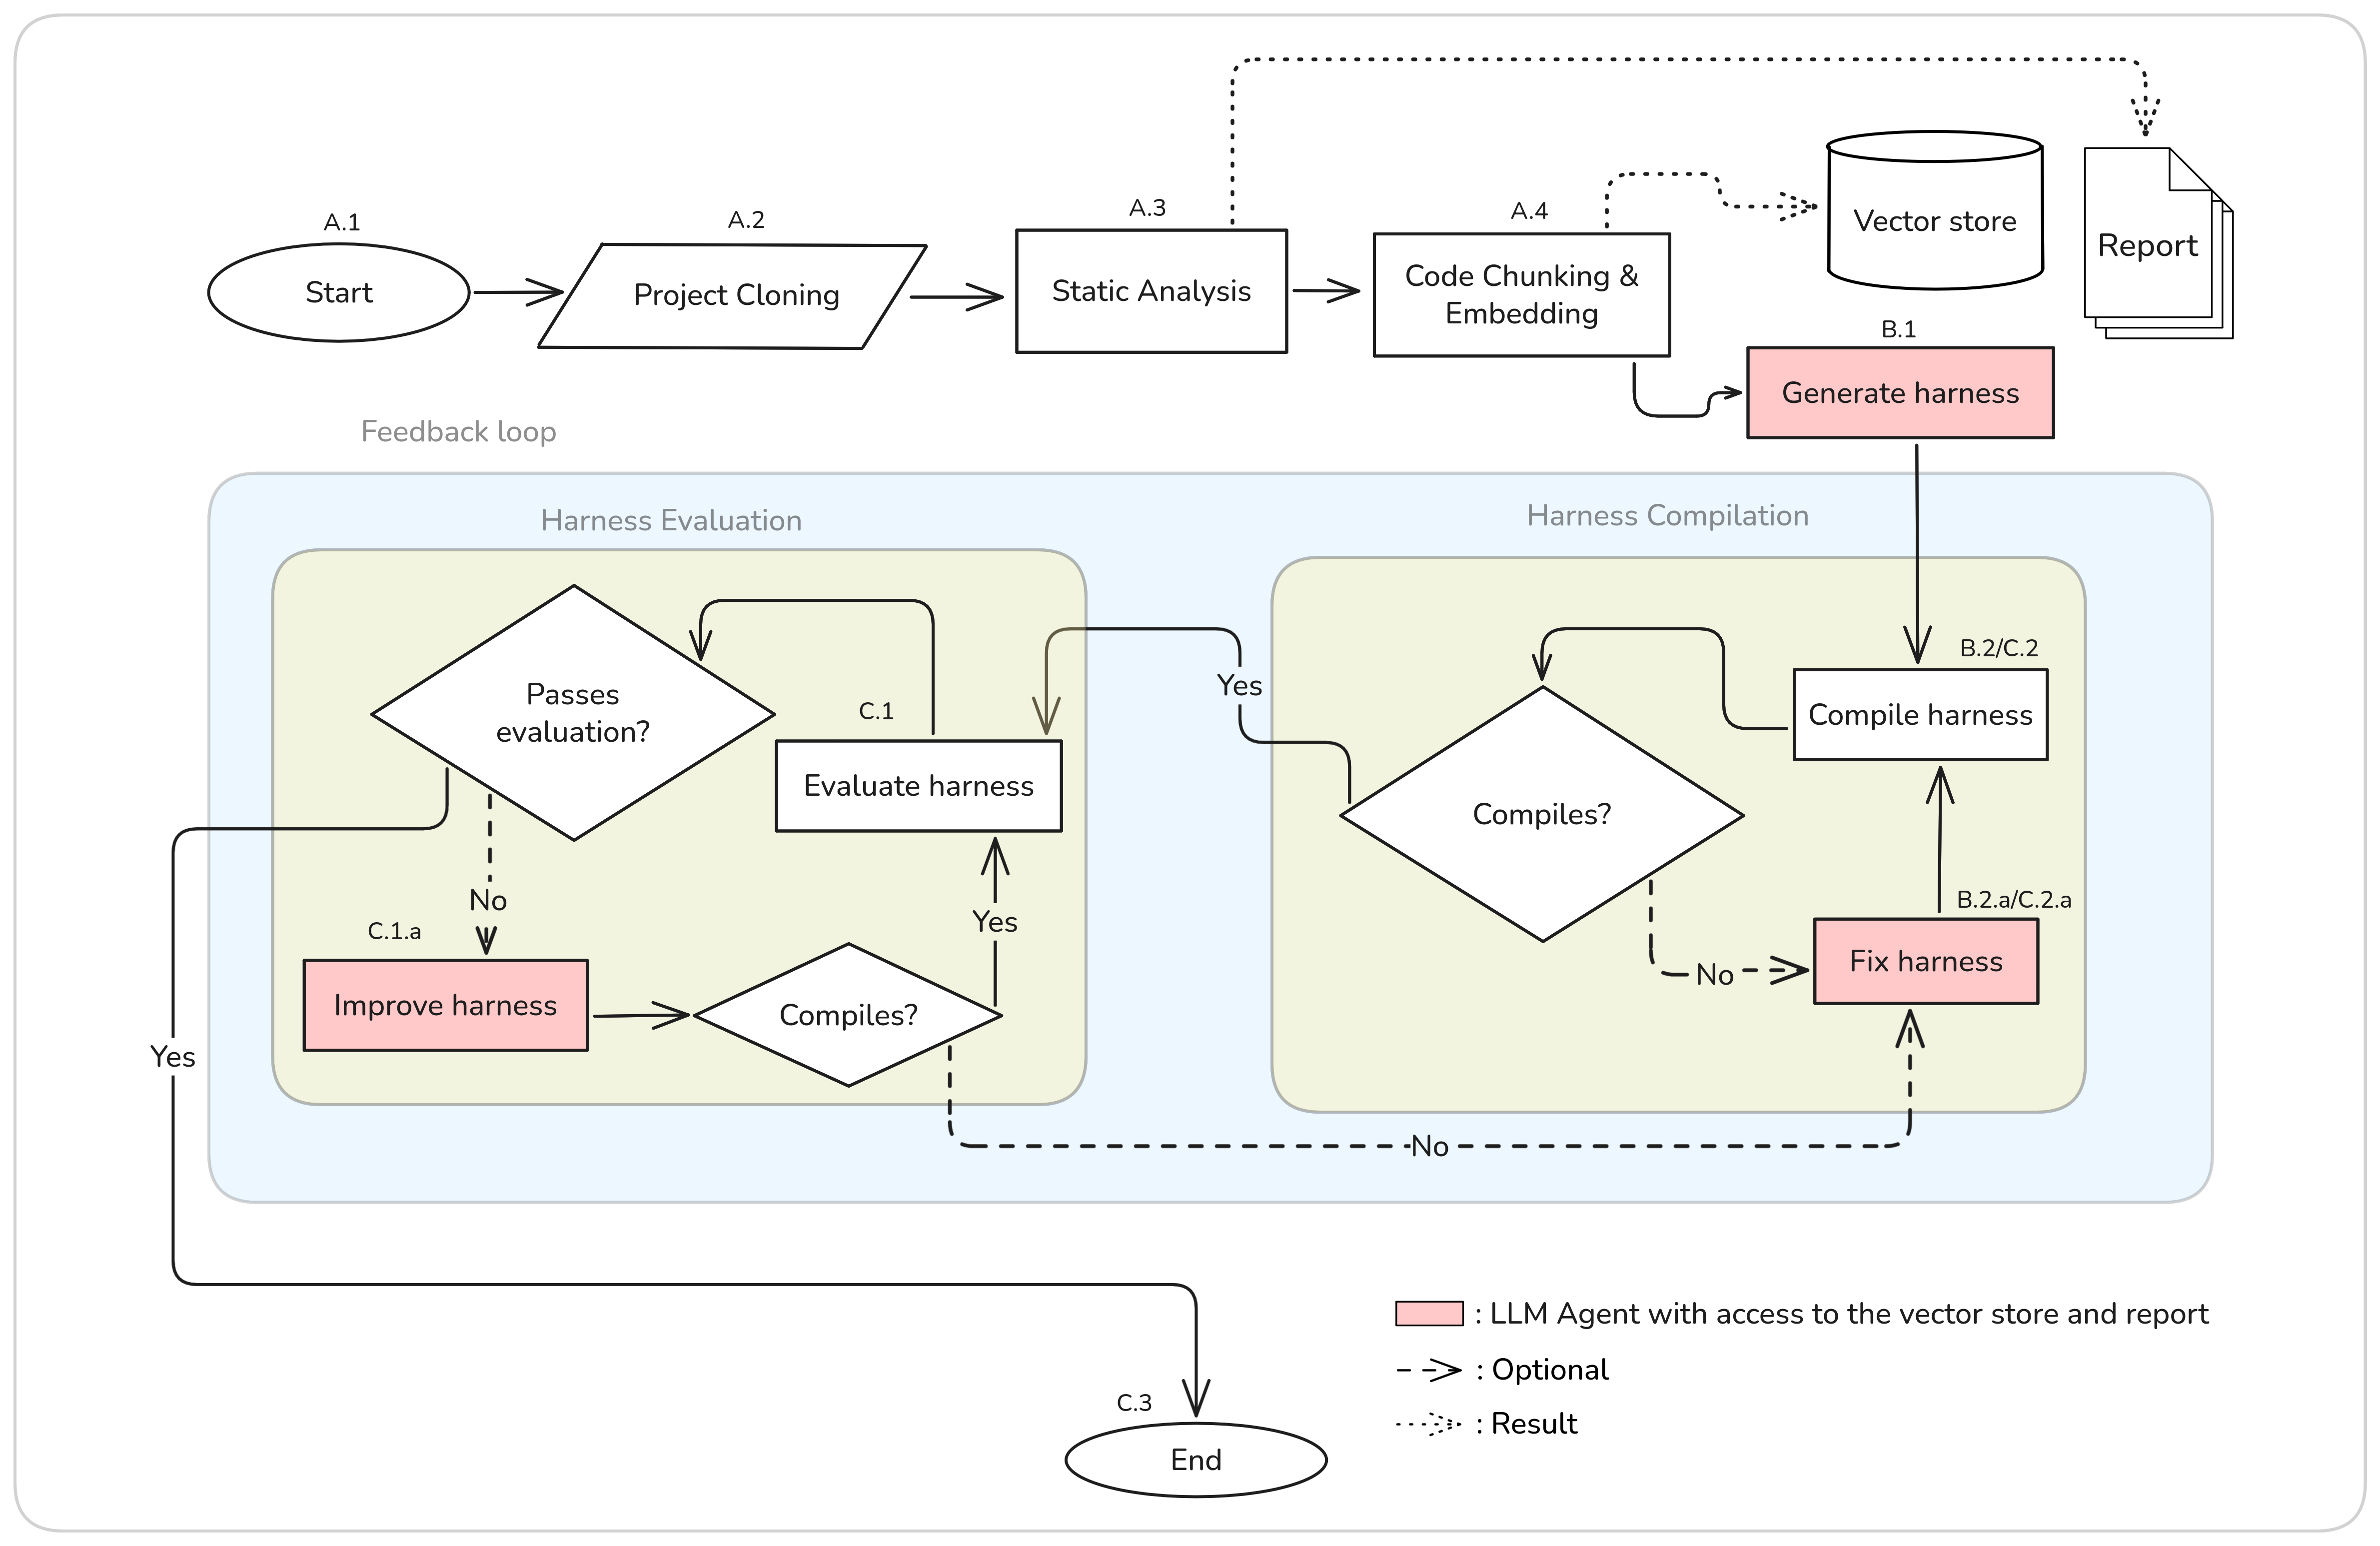
\includegraphics[keepaspectratio]{chapters/../resources/flowchart.png}}

}

\caption[OverHAuL Workflow]{\label{fig-flowchart}Overview of OverHAuL's
automatic harnessing process.}

\end{figure}%

As detailed in Section~\ref{sec-differences}, OverHAuL does not expect
and depend on the existence of client code or unit tests
\autocite{utopia,fudge,fuzzgen} \emph{nor} does it require any
preexisting fuzzing harnesses \autocite{oss-fuzz-gen} or any
documentation present \autocite{sun2024}. Also importantly, OverHAuL is
decoupled from other fuzzing projects, thus lowering the barrier to
entry for new projects \autocite{oss-fuzz-gen,oss-fuzz}. Lastly, the
user isn't mandated to manually specify the function which the
harness-to-be-generated must fuzz. Instead, OverHAuL's agents examine
and assess the provided codebase, choosing after evaluation the most
optimal target function.

OverHAuL utilizes autonomous ReAct agents which inspect and analyze the
project's source code. The latter is stored and interacted with as a set
of text embeddings \autocite{mikolov2013}, kept in a vector store. Both
approaches are, to the best of our knowledge, novel in the field of
automatic fuzzing harnesses generation. OverHAuL also implements an
evaluation component that assesses in real-time all generated harnesses,
making the results tenable, reproducible and well-founded. Ideally, this
methodology provides a comprehensive and systematic framework for
identifying previously unknown software vulnerabilities in projects that
have not yet been fuzz tested.

Finally, OverHAuL excels in its user-friendliness, as it constitutes a
simple and easily-installable Python package with minimal external
dependencies---only real dependency being Clang, a prevalent compiler
available across all primary operating systems. This contrasts most
other comparable systems, which are typically characterized by their
limited documentation, lack of extensive testing, and a focus primarily
on experimental functionality.

\section{Architecture}\label{sec-architecture}

OverHAuL can be compartmentalized in three stages: First, the project
analysis stage (Section~\ref{sec-analysis}), the harness creation stage
(Section~\ref{sec-creation}) and the harness evaluation stage
(Section~\ref{sec-evaluation}).

\subsection{Project Analysis}\label{sec-analysis}

In the project analysis stage (steps A.1--A.4), the project to be fuzzed
is ran through a static analysis tool and is sliced into function-level
chunks, which are stored in a vector store. The results of this stage
are a static analysis report and a vector store containing embeddings of
function-level code chunks, both of which are later available to the LLM
agents.

The static analysis tool Flawfinder \autocite{flawfinder} is executed
with the project directory as input and is responsible for the static
analysis report. This report is considered a meaningful resource, since
it provides the LLM agent with some starting points to explore,
regarding the occurrences of potentially vulnerable functions and/or
unsafe code practices.

The vector store is created in the following manner: The codebase is
first chunked in function-level pieces by traversing the code's Abstract
Syntax Tree (AST) through Clang. Each chunk is represented by an object
with the function's signature, the corresponding filepath and the
function's body. Afterwards, each function body is turned into a vector
embedding through an embedding model. Each embedding is stored in the
vector store. This structure is created and used for easier and more
semantically meaningful code retrieval, and to also combat context
window limitations present in LLMs.

\subsection{Harness Creation}\label{sec-creation}

Second is the harness creation stage (steps B.1--B.2). In this part, a
``generator'' ReAct LLM agent is tasked with creating a fuzzing harness
for the project. The agent has access to a querying tool that acts as an
interface between it and the vector store. When the agent makes queries
like ``functions containing \texttt{strcpy()}'', the querying tool turns
the question into an embedding and through similarity search returns the
top \(k=5\) most similar results---in this case, functions of the
project. With this approach, the agent is able to explore the codebase
semantically and pinpoint potentially vulnerable usage patterns easily.

The harness generated by the agent is then compiled using Clang and
linked with the AddressSanitizer, LeakSanitizer, and
UndefinedBehaviorSanitizer. The compilation command used is generated
programmatically, according to the rules described in
Section~\ref{sec-scope}. If the compilation fails for any reason, e.g.~a
missing header include, then the generated faulty harness and its
compilation output are passed to a new ``fixer'' agent tasked with
repairing any errors in the harness (step B.2.a). This results in a
newly generated harness, presumably free from the previously shown
flaws. This process is iterated until a compilable harness has been
obtained. After success, a script is also exported in the project
directory, containing the generated compilation command.

\subsection{Harness Evaluation}\label{sec-evaluation}

Third comes the evaluation stage (steps C.1--C.3). During this step, the
compiled harness is executed and its results evaluated. Namely, a
generated harness passes the evaluation phase if and only if:

\begin{enumerate}
\def\labelenumi{\arabic{enumi}.}
\item
  The harness has no memory leaks during its execution

  This is inferred by the existence of
  \texttt{leak-\textless{}hash\textgreater{}} files.
\item
  A new testcase was created \emph{or} the harness executed for at least
  \texttt{MIN\_EXECUTION\_TIME} (i.e.~did not crash on its own)

  When a crash happens, and thus a testcase is created, it results in a
  \texttt{crash-\textless{}hash\textgreater{}} file.
\item
  The created testcase is not empty

  This is examined through xxd's output given the crash-file.
\end{enumerate}

Similarly to the second stage's compilation phase (steps B.2--B.2.a), if
a harness does not pass the evaluation for whatever reason it is sent to
an ``improver'' agent. This agent is instructed to refine it based on
its code and cause of failing the evaluation. This process is also
iterative. If any of the improved harness versions fail to compile, the
aforementioned ``fixer'' agent is utilized again (steps C.2--C.2.a). All
produced crash files and the harness execution output are saved in the
project's directory.

\section{OverHAuL Techniques}\label{sec-techniques}

The fundamental techniques that distinguish OverHAuL in its approach and
enhance its effectiveness in achieving its objectives are: The
implementation of an iterative feedback loop between the LLM agents, the
distribution of responsibility across a triplet of distinct agents and
the employment of a ``codebase oracle'' for interacting with the given
project's source code.

\subsection{Feedback Loop}\label{sec-loop}

The initial generated harness produced by OverHAuL is unlikely to be
successful from the get-go. The iterative feedback loop implemented
facilitates its enhancement, enabling the harness to be tested under
real-world conditions and subsequently refined based on the results of
these tests. This approach mirrors the typical workflow employed by
developers in the process of creating and optimizing fuzz targets.

In this iterative framework, the development process continues until
either an acceptable and functional harness is realized or the defined
\emph{iteration budget} is exhausted. The iteration budget \(N=10\) is
initialized at the onset of OverHAuL's execution and is shared between
both the compilation and evaluation phases of the harness development
process. This means that the iteration budget is decremented each time a
dashed arrow in the flowchart illustrated in Figure~\ref{fig-flowchart}
is followed. Such an approach allows for targeted improvements while
maintaining oversight of resource allocation throughout the harness
development cycle.

\subsection{React Agents Triplet}\label{react-agents-triplet}

An integral design decision in our framework is the implementation of
each agent as a distinct LLM instance, although all utilizing the same
underlying model. This approach yields several advantages, particularly
in the context of maintaining separate and independent contexts for each
agent throughout each OverHAuL run.

By assigning individual contexts to the agents, we enable a broader
exploration of possibilities during each run. For instance, the
``improver'' agent can investigate alternative pathways or strategies
that the ``generator'' agent may have potentially overlooked or
internally deemed inadequate inaccurately. This separation not only
fosters a more diverse range of solutions but also enhances the overall
robustness of the system by allowing for iterative refinement based on
each agent's unique insights.

Furthermore, this design choice effectively addresses the limitations
imposed by context window sizes. By distributing the ``cognitive'' load
across multiple agents, we can manage and mitigate the risks associated
with exceeding these constraints. As a result, this architecture
promotes efficient utilization of available resources while maximizing
the potential for innovative outcomes in multi-agent interactions. This
layered approach ultimately contributes to a more dynamic and
exploratory research environment, facilitating a comprehensive
examination of the problem space.

\subsection{Codebase Oracle}\label{sec-oracle}

The third central technique employed is the creation and utilization of
a codebase oracle, which is effectively realized through a vector store.
This oracle is designed to contain the various functions within the
project, enabling it to return the most semantically similar functions
upon querying it. Such an approach serves to address the inherent
challenges associated with code exploration difficulties faced by LLM
agents, particularly in relation to their limited context window.

By structuring the codebase into chunks at the level of individual
functions, LLM agents can engage with the code more effectively by
focusing on its functional components. This methodology not only allows
for a more nuanced understanding of the codebase but also ensures that
the responses generated do not consume an excessive portion of the
limited context window available to the agents. In contrast, if the
codebase were organized and queried at the file level, the chunks of
information would inevitably become larger, leading to an increase in
noise and a dilution of meaningful content in each chunk
\autocite{zhao2024}. Given the constant size of the embeddings used in
processing, each progressively larger chunk would be less semantically
significant, ultimately compromising the quality of the retrieval
process.

Defining the function as the primary unit of analysis represents the
most proportionate balance between the size of the code segments and
their semantic significance. It serves as the ideal ``zoom-in'' level
for the exploration of code, allowing for greater clarity and precision
in understanding the functionality of individual code segments. This
same principle is widely recognized in the training of code-specific
LLMs, where a function-level approach has been shown to enhance
performance and comprehension \autocite{chen2021}. By adopting this
methodology, we aim to foster a more robust interaction between LLM
agents and the underlying codebase, ultimately facilitating a more
effective and efficient exploration process.

\section{High-Level Algorithm}\label{high-level-algorithm}

A pseudocode version of OverHAuL's main function can be seen in
Algorithm~\ref{alg-main}. It represents the workflow presented in
Figure~\ref{fig-flowchart} and uses the techniques described in sections
\ref{sec-architecture} and \ref{sec-techniques}. It is important to
emphasize that, within the context of this algorithm, the
\texttt{HarnessAgents()} function serves as an interface that bridges
the ``generator'', ``fixer'' and ``improver'' LLM agents. The agent that
is used upon each function call depends on the values of the function's
arguments. This results in the \(harness\) variable representing all
generated, fixed or improved harnesses. This approach is adopted for
making the abstract algorithm simpler and easier to understand.

\begin{algorithm}[H]
\caption{OverHAuL}
\label{alg-main}
\begin{algorithmic}[1]
\Require $repository$
\Ensure $harness, compilation\_script, crash\_input, execution\_log$
  \State $path \gets$ \Call{RepoClone}{$repository$}
  \State $report \gets$ \Call{StaticAnalysis}{$path$}
  \State $vector\_store \gets$ \Call{CreateOracle}{$path$}
  \State $acceptable \gets$ False
  \State $compiled \gets$ False
  \State $error \gets$ None
  \State $violation \gets$ None
  \State $output \gets$ None
  \For{$i = 1$ to $MAX\_ITERATIONS$}
    \State $harness \gets$ \Call{HarnessAgents}{$path, report, vector\_store, error, violation, output$}
    \State $error, compiled \gets$ \Call{BuildHarness}{$path, harness$}
    \If{$\neg compiled$}
      \State \textbf{continue} \Comment{Fix harness}
    \EndIf
    \State $output, accepted \gets $\Call{EvaluateHarness}{$path, harness$}
    \If{$\neg accepted$}
      \State \textbf{continue} \Comment{Improve harness}
    \Else
      \State $acceptable \gets$ True
      \State \textbf{break}
    \EndIf
  \EndFor
  \State \Return $compiled \land acceptable$
\end{algorithmic}
\end{algorithm}

\section{Installation and Usage}\label{sec-install}

The source code of OverHAuL is available in
\url{https://github.com/kchousos/OverHAuL}. OverHAuL can be installed by
cloning the git repository locally, creating and enabling a Python3.10
virtual environment \autocite{venv} and installing it inside the
environment using Python's PIP package installer \autocite{pip}, like in
Listing~\ref{lst-install}.

\begin{codelisting}

\caption[OverHAuL installation]{\label{lst-install}OverHAuL's
installation process.}

\centering{

\begin{Shaded}
\begin{Highlighting}[numbers=left,,]
\NormalTok{$ git clone https://github.com/kchousos/overhaul; cd overhaul}
\NormalTok{  ...}
\NormalTok{$ python3.10 {-}m venv .venv}
\NormalTok{$ source ./.venv/bin/activate}
\NormalTok{$ pip install .}
\NormalTok{  ...}
\NormalTok{$ overhaul {-}{-}help}
\NormalTok{usage: overhaul [{-}h] [{-}c COMMIT] [{-}m MODEL] [{-}f FILES [FILES ...]] [{-}o OUTPUT\_DIR] repo}

\NormalTok{Generate fuzzing harnesses for C/C++ projects}

\NormalTok{positional arguments:}
\NormalTok{  repo                  Link of a project\textquotesingle{}s git repo, for which to generate a harness.}

\NormalTok{options:}
\NormalTok{  {-}h, {-}{-}help            show this help message and exit}
\NormalTok{  {-}c COMMIT, {-}{-}commit COMMIT}
\NormalTok{                        A specific commit of the project to check out}
\NormalTok{  {-}m MODEL, {-}{-}model MODEL}
\NormalTok{                        LLM model to be used. Available: o3{-}mini, o3, gpt{-}4o,}
\NormalTok{                        gpt{-}4o{-}mini, gpt{-}4.1, gpt{-}4.1{-}mini, gpt{-}3.5{-}turbo, gpt{-}4}
\NormalTok{  {-}f FILES [FILES ...], {-}{-}files FILES [FILES ...]}
\NormalTok{                        File patterns to include in analysis (e.g. *.c *.h)}
\NormalTok{  {-}o OUTPUT\_DIR, {-}{-}output{-}dir OUTPUT\_DIR}
\NormalTok{                        Directory to clone the project into. Defaults to "output"}
\NormalTok{$}
\end{Highlighting}
\end{Shaded}

}

\end{codelisting}%

To use OverHAuL, you need to provide a secret key for using OpenAI's API
service. This key can be either stored in a \texttt{.env} file in the
root directory, like so:

\begin{Shaded}
\begin{Highlighting}[numbers=left,,]
\NormalTok{\# cat .env}
\NormalTok{OPENAI\_API\_KEY=\textless{}API{-}key{-}here\textgreater{}}
\end{Highlighting}
\end{Shaded}

Or it can be exported in the shell environment:

\begin{Shaded}
\begin{Highlighting}[numbers=left,,]
\NormalTok{$ export OPENAI\_API\_KEY=\textless{}API{-}key{-}here\textgreater{}}
\NormalTok{$ overhaul \textless{}repo{-}link\textgreater{}}
\end{Highlighting}
\end{Shaded}

Once these preliminary steps are completed, OverHAuL can be executed.
The primary argument required by OverHAuL is the repository link of the
library that is to be fuzzed. Additionally, users have the option to
specify certain command-line flags, which allow them to control the
checked-out commit of the cloned project, select the OpenAI LLM model
from a predefined list, define specific file patterns for OverHAuL to
search for, and determine the directory in which the project will be
cloned. A sample successful execution can is presented in
Figure~\ref{fig-success}.

\begin{figure}

\centering{

\pandocbounded{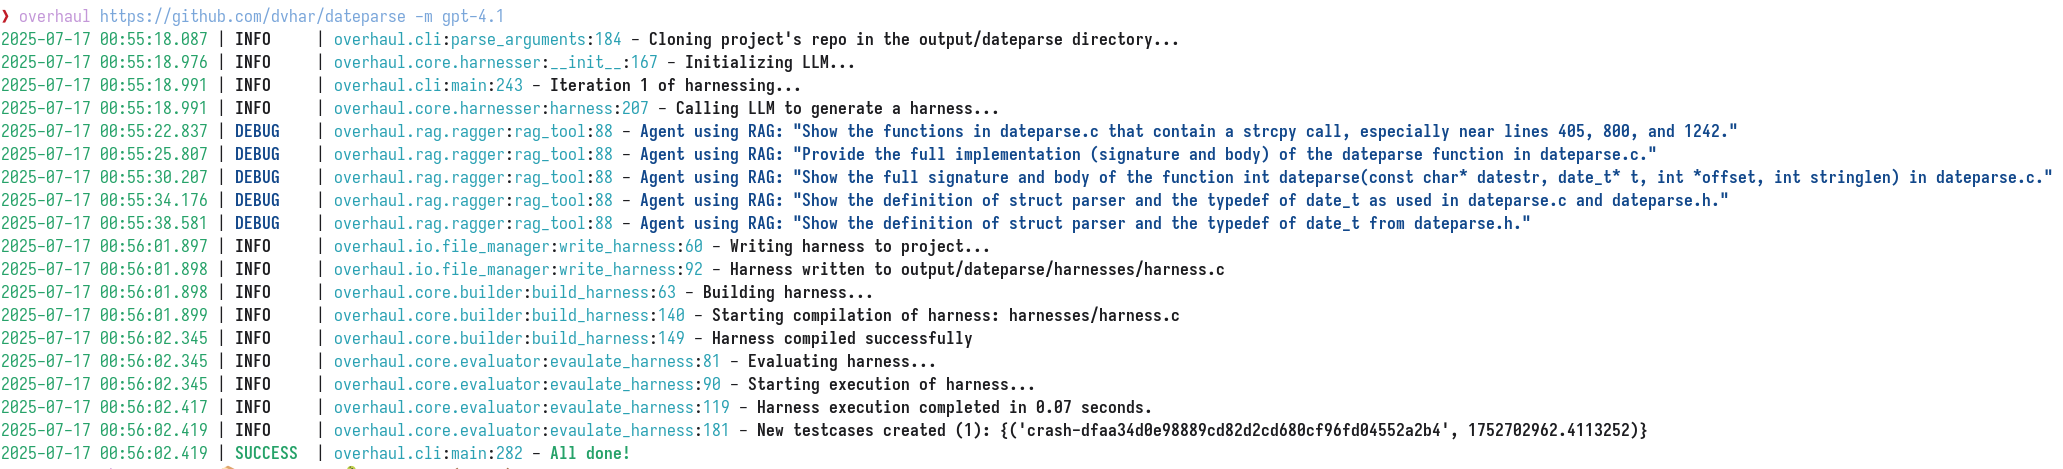
\includegraphics[keepaspectratio]{chapters/../resources/successful-execution.png}}

}

\caption[OverHAuL execution example]{\label{fig-success}A successful
execution of OverHAuL, harnessing
\href{https://github.com/dvhar/dateparse}{dvhar's dateparsing C
library}, using OpenAI's gpt-4.1 model. Debug statements are printed to
showcase the interaction between the LLM agents and the codebase oracle
(Section~\ref{sec-oracle}).}

\end{figure}%

In this example, the dateparse repository is cloned into the
\texttt{./output/dateparse} directory, which is relative to the root
directory of OverHAuL. Following a successful execution, this directory
will contain a new folder named \texttt{harnesses}, which will house all
the generated harnesses formatted as \texttt{harness\_n.c}---where \(n\)
ranges from 1 to \(N-1\), with \(N\) representing the total number of
harnesses produced. The most recent and verifiably correct harness will
be designated simply as \texttt{harness.c}. Additionally, the dateparse
directory will include an executable script named \texttt{overhaul.sh},
which contains the compilation command necessary for the harness. A log
file titled \texttt{harness.out} will also be present, documenting the
output from the latest harness execution. Lastly and most importantly,
there will be at least one non-empty crash file included, serving as a
witness to the harness's correctness.

\section{Scope}\label{sec-scope}

Currently, OverHAuL is designed to generate new harnesses specifically
for medium-sized C libraries. Given the inherent complexity of dealing
with C++ projects, this is not a feature yet supported within the
system.

The compilation command utilized by OverHAuL is created
programmatically. It incorporates the root directory along with all
subdirectories that conform to a predefined set of common naming
conventions. Additionally, the compilation process uses all C source
files identified within these directories. Crucially, it is important
that no \texttt{main()} function is present in any of the files to
ensure successful compilation. For this reason any files or directories
that include ``test'', ``main'', ``example'', ``demo'', or ``benchmark''
in their paths are systematically excluded from the compilation process.
This exclusion also decreases the ``noise'' in the oracle, as these
files do not constitute part of the core library and would therefore not
contain any functions meaningful to the LLM agents.

Lastly, No support for build systems such as Make or CMake
\autocite{cedilnik2000,feldman1979} is yet implemented. Such
functionality would exponentially increase the complexity of the build
step and is beyond the scope of this thesis.

\bookmarksetup{startatroot}

\chapter{Implementation}\label{sec-implementation}

In creating the codebase oracle, we employ the ``libclang'' Python
package \autocite{he2025} to slice functions based on the AST capability
provided by Clang. As detailed in Section~\ref{sec-oracle}, the
intermediate output consists of a list of Python dictionaries, with each
dictionary storing a function's body, signature, and corresponding file
path. Each chunk of function code is then converted into an embedding
using OpenAI's ``text-embedding-3-small'' model
\autocite{openaidocs2025a} and stored in a FAISS vector store index
\autocite{faiss}. This index is mapped to a metadata structure that
contains the aforementioned function data---specifically the actual
function body, signature, and file path. When a search is conducted on
the index, the results returned are the embeddings. The responses that
the LLM agent receives are derived from the corresponding metadata
entries of each embedding.

All LLM agents and components are developed using the DSPy library, a
declarative Python framework for LLM programming created by Stanford's
NLP research team \autocite{dspy}. DSPy offers built-in modules and
abstractions that facilitate the composition of LLMs and prompting
techniques, such as Chain of Thought and ReAct (Listing~\ref{lst-dspy}).
Each agent within OverHAuL is an instance of DSPy's ReAct module
\autocite{stanfordnlpteam2025}, accompanied by a custom Signature
\autocite{stanfordnlpteam2025a}---displayed in
Appendix~\ref{sec-signatures}. DSPy was selected over other contemporary
LLM libraries, such as LangChain and Llamaindex
\autocite{langchain,llamaindex}, because of its user-friendliness,
logical abstractions, and efficient development process---qualities that
are often lacking in these alternative libraries
\autocite{both2024,woolf2023,woyera2023}.

\begin{codelisting}

\caption[DSPy example]{\label{lst-dspy}Sample DSPy program.}

\centering{

\begin{Shaded}
\begin{Highlighting}[numbers=left,,]
\ImportTok{import}\NormalTok{ dspy}
\NormalTok{lm }\OperatorTok{=}\NormalTok{ dspy.LM(}\StringTok{\textquotesingle{}openai/gpt{-}4o{-}mini\textquotesingle{}}\NormalTok{, api\_key}\OperatorTok{=}\StringTok{\textquotesingle{}YOUR\_OPENAI\_API\_KEY\textquotesingle{}}\NormalTok{)}
\NormalTok{dspy.configure(lm}\OperatorTok{=}\NormalTok{lm)}

\NormalTok{math }\OperatorTok{=}\NormalTok{ dspy.ChainOfThought(}\StringTok{"question {-}\textgreater{} answer: float"}\NormalTok{)}
\NormalTok{math(question}\OperatorTok{=}\StringTok{"Two dice are tossed. What is the probability that the sum equals two?"}\NormalTok{)}
\end{Highlighting}
\end{Shaded}

}

\end{codelisting}%

Repository cloning is executed using the \texttt{-\/-depth\ 1} flag to
minimize disk storage usage and reduce the size of artifacts.

The current implementation of OverHAuL sits at 1,254 source lines of
Python code.

\section{Development Tools}\label{development-tools}

The development of OverHAuL incorporates a variety of tools aimed at
enhancing functionality and efficiency. Notably, ``uv'' is a Python
package and project manager written in Rust that serves as a replacement
for Poetry. Additionally, ``Ruff,'' a code linter and formatter also
developed in Rust, contributes to code quality by enforcing consistent
formatting standards. The project also employs ``MyPy,'' the widely-used
static type checker for Python, to ensure type correctness. Testing is
facilitated through ``PyTest,'' a robust Python testing framework.
Lastly, ``pdoc'' is utilized as a Static Site Generator (SSG) to
automate the creation of API documentation\footnote{\url{https://kchousos.github.io/OverHAuL/}}
\autocite{astral2025,astral2025a,cortesi2025,pytestdevteam2025,pythonsoftwarefoundation2025}.

\section{Reproducibility}\label{reproducibility}

OverHAuL's source code is available at
\url{https://github.com/kchousos/OverHAuL}. Each benchmark run was
conducted within the framework of a GitHub Actions workflow, resulting
in a detailed summary accompanied by an artifact containing all cloned
repositories. These artifacts are the compressed result directories
described in Section~\ref{sec-local} and provide the essential
components necessary for the reproducibility each project's results, as
described in Section~\ref{sec-install}. All benchmark runs can be
conveniently accessed at
\url{https://github.com/kchousos/OverHAuL/actions/workflows/benchmarks.yml}.

\bookmarksetup{startatroot}

\chapter{Evaluation}\label{sec-eval}

To thoroughly assess the performance and effectiveness of OverHAuL, we
established four \emph{research questions} to direct our investigative
efforts. These questions are designed to provide a structured framework
for our inquiry and to ensure that our research remains focused on the
key aspects of OverHAuL's functionality and impact within its intended
domain. By addressing these questions, we aim to uncover valuable
insights that will contribute to a deeper understanding of OverHAuL's
capabilities and its position in contemporary automatic fuzzing
applications:

\begin{itemize}
\item
  \textbf{RQ1}: Can OverHAuL generate working harnesses for unfuzzed C
  projects?
\item
  \textbf{RQ2}: What characteristics do these harnesses have? Are they
  similar to man-made harnesses?
\item
  \textbf{RQ3}: How do LLM usage patterns influence the generated
  harnesses?
\item
  \textbf{RQ4}: How do different symbolic techniques affect the
  generated harnesses?
\end{itemize}

\section{Experimental Benchmark}\label{sec-benchmark}

To evaluate OverHAuL, a benchmarking script was implemented\footnote{\url{https://github.com/kchousos/OverHAuL/blob/master/benchmarks/benchmark.sh}}
and a corpus of ten open-source C libraries was assembled. This
collection comprises of: Firstly, GitHub user dhvar's dateparse library,
which is also used as a running example in OSS-Fuzz-Gen's
\autocite{oss-fuzz-gen} experimental from-scratch harnessing feature
(Section~\ref{sec-ofg}). Secondly, nine other libraries chosen
randomly\footnote{From the subset of libraries that do not have exotic
  external dependencies, like the X11 development toolchain.} from the
package catalog of Clib, a ``package manager for the C programming
language'' \autocite{clibs,clib}. All libraries can be seen
Table~\ref{tbl-projects}, along with their descriptions.

\begin{longtable}[]{@{}
  >{\raggedright\arraybackslash}p{(\linewidth - 6\tabcolsep) * \real{0.4367}}
  >{\raggedright\arraybackslash}p{(\linewidth - 6\tabcolsep) * \real{0.4810}}
  >{\raggedleft\arraybackslash}p{(\linewidth - 6\tabcolsep) * \real{0.0443}}
  >{\raggedleft\arraybackslash}p{(\linewidth - 6\tabcolsep) * \real{0.0380}}@{}}
\caption{The benchmark project corpus. Each project name links to its
corresponding GitHub repository. Each is followed by a short description
and its GitHub stars count, as of July 18th,
2025.}\label{tbl-projects}\tabularnewline
\toprule\noalign{}
\begin{minipage}[b]{\linewidth}\raggedright
Project
\end{minipage} & \begin{minipage}[b]{\linewidth}\raggedright
Description
\end{minipage} & \begin{minipage}[b]{\linewidth}\raggedleft
Stars
\end{minipage} & \begin{minipage}[b]{\linewidth}\raggedleft
SLOC
\end{minipage} \\
\midrule\noalign{}
\endfirsthead
\toprule\noalign{}
\begin{minipage}[b]{\linewidth}\raggedright
Project
\end{minipage} & \begin{minipage}[b]{\linewidth}\raggedright
Description
\end{minipage} & \begin{minipage}[b]{\linewidth}\raggedleft
Stars
\end{minipage} & \begin{minipage}[b]{\linewidth}\raggedleft
SLOC
\end{minipage} \\
\midrule\noalign{}
\endhead
\bottomrule\noalign{}
\endlastfoot
\href{https://github.com/dvhar/dateparse}{dvhar/dateparse} & A library
that allows parsing dates without knowing the format in advance. & 2 &
2272 \\
\href{https://github.com/clibs/buffer}{clibs/buffer} & A string
manipulation library. & 204 & 354 \\
\href{https://github.com/jwerle/libbeaufort}{jwerle/libbeaufort} & A
library implementation of the Beaufort cipher \autocite{franksen1993}. &
13 & 321 \\
\href{https://github.com/jwerle/libbacon}{jwerle/libbacon} & A library
implementation of the Baconian cipher \autocite{bacon1861}. & 8 & 191 \\
\href{https://github.com/jwerle/chfreq.c}{jwerle/chfreq.c} & A library
for computing the character frequency in a string. & 5 & 55 \\
\href{https://github.com/jwerle/progress.c}{jwerle/progress.c} & A
library for displaying progress bars in the terminal. & 76 & 357 \\
\href{https://github.com/willemt/cbuffer}{willemt/cbuffer} & A circular
buffer implementation. & 261 & 170 \\
\href{https://github.com/willemt/torrent-reader}{willemt/torrent-reader}
& A torrent-file reader library. & 6 & 294 \\
\href{https://github.com/orangeduck/mpc}{orangeduck/mpc} & A
type-generic parser combinator library. & 2,753 & 3632 \\
\href{https://github.com/h2non/semver.c}{h2non/semver.c} & A semantic
version v2.0 parsing and rendering library \autocite{semver}. & 190 &
608 \\
\end{longtable}

\subsection{Local Benchmarking}\label{sec-local}

To run the benchmark locally, one would need to follow the installation
instructions in Section~\ref{sec-install} and then execute the
benchmarking script, like so:

\begin{Shaded}
\begin{Highlighting}[numbers=left,,]
\NormalTok{$ ./benchmarks/benchmark.sh}
\end{Highlighting}
\end{Shaded}

The cloned repositories with their corresponding harnesses will then be
located in a subdirectory of \texttt{benchmark\_results}, which will
have the name format of
\texttt{mini\_\_\textless{}timestamp\textgreater{}\_\_ReAct\_\_\textless{}llm-model\textgreater{}\_\_\textless{}max-exec-time\textgreater{}\_\_\textless{}iter-budget\textgreater{}}.
``Mini'' corresponds to the benchmark project corpus described above,
since a 30-project corpus was initially created and is now coined as
``full'' benchmark. Both the mini and full benchmarks are located in
\texttt{benchmarks/repos.txt} and \texttt{benchmarks/repos-mini.txt}
respectively. To execute the benchmark for the ``full'' corpus, users
can add the \texttt{-b\ full} flag in the script's invocation. Also, the
LLM model used can be defined with the \texttt{-m} command-line flag.

\bookmarksetup{startatroot}

\chapter{Results}\label{sec-results}

OverHAuL was evaluated through the experimental benchmark
(Section~\ref{sec-benchmark}) from 6th of June, 2025 to 18th of July,
2025, using OpenAI's gpt-4.1-mini model \autocite{openaidocs2025}. For
these runs, each OverHAuL execution was configured with a 5 minute
harness execution timeout and an iteration budget of 10. Each benchmark
run was executed as a GitHub Actions workflow, and the result directory
(described in Section~\ref{sec-local}) for each is available as a
downloadable artifact in the corresponding GitHub Actions entry. In
Figure~\ref{fig-results}, the results of these benchmark runs are
showcased.

\begin{figure}

\centering{

\pandocbounded{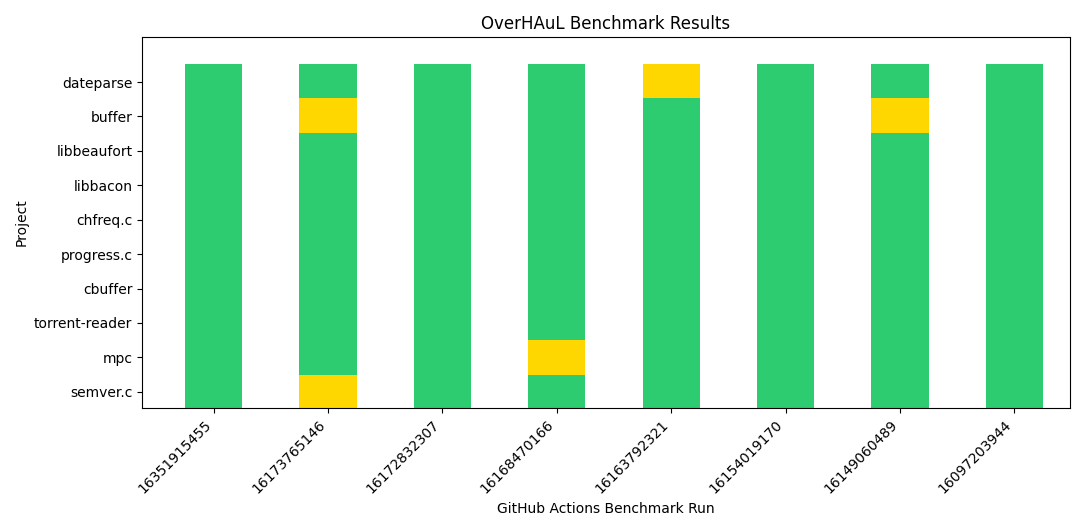
\includegraphics[keepaspectratio]{chapters/../resources/results.png}}

}

\caption[Benchmark Results]{\label{fig-results}The benchmark results for
OverHAuL are illustrated with the \(y\)-axis depicting the ten-project
corpus outlined in Section~\ref{sec-benchmark}. The \(x\)-axis
represents the various benchmark runs. Each label constitutes a unique
hash identifier corresponding to a specific GitHub Actions workflow run,
which can be accessed at
\url{https://github.com/kchousos/OverHAuL/actions/runs/HASH}. An
overview of all benchmark runs is available at
\url{https://github.com/kchousos/OverHAuL/actions/workflows/benchmarks.yml}.
In this matrix, a green/1 block indicates that OverHAuL successfully
generated a new harness for the project and was able to find a crash
input. On the other hand, an orange/0 block indicates that while a
compilable harness was produced, no crash input was found within the
five-minute execution period. Importantly, there are no red/-1 blocks,
which would indicate cases where a compilable harness could not be
generated.}

\end{figure}%

\section{Answers to RQs}\label{answers-to-rqs}

We can deduce the following facts from Figure~\ref{fig-results}:
Firstly, OverHAuL has a very high success rate in finding crash inputs
for the given programs, specifically one of \textbf{92.5\%}. Secondly,
although according strictly to these results OverHAuL never generates an
un-compilable harness, we can err on the side of caution and infer that
OverHAuL not being able to generate a compilable harness is a rare
occurrence. These conclusions can safely answer RQ1 with a resounding
yes.

From sampling OverHAuL's generated harnesses, the answer to RQ2 remains
unclear. Most of the time, the fuzz targets that are produced are
understandable and similar to something a software engineer might
program. Take for example Listing~\ref{lst-sample-dateparse}.
Nonetheless, sometimes generated harnesses contain usage of inexplicable
or arbitrary constants and peculiar control flow checks. This makes them
harder to understand and quite possibly incorrect in many cases, thus
diverging from seeming human-written. RQ2's answer remains an unclear
``it depends'', given the variance in OverHAuL's results.

\begin{codelisting}

\caption[Sample dateparse harness]{\label{lst-sample-dateparse}Sample
harness for dateparse, generated by OverHAuL.}

\centering{

\begin{Shaded}
\begin{Highlighting}[numbers=left,,]
\PreprocessorTok{\#include }\ImportTok{\textless{}stddef.h\textgreater{}}
\PreprocessorTok{\#include }\ImportTok{\textless{}stdint.h\textgreater{}}
\PreprocessorTok{\#include }\ImportTok{\textless{}string.h\textgreater{}}
\PreprocessorTok{\#include }\ImportTok{\textless{}stdlib.h\textgreater{}}
\PreprocessorTok{\#include }\ImportTok{"dateparse.h"}

\CommentTok{// No artificial size limit to allow fuzzer to explore full input size for boundaries}

\DataTypeTok{int}\NormalTok{ LLVMFuzzerTestOneInput}\OperatorTok{(}\DataTypeTok{const} \DataTypeTok{uint8\_t} \OperatorTok{*}\NormalTok{data}\OperatorTok{,} \DataTypeTok{size\_t}\NormalTok{ size}\OperatorTok{)} \OperatorTok{\{}
    \CommentTok{// Allocate buffer with extra byte for null termination}
    \DataTypeTok{char} \OperatorTok{*}\NormalTok{input\_str }\OperatorTok{=} \OperatorTok{(}\DataTypeTok{char} \OperatorTok{*)}\NormalTok{malloc}\OperatorTok{(}\NormalTok{size }\OperatorTok{+} \DecValTok{1}\OperatorTok{);}
    \ControlFlowTok{if} \OperatorTok{(!}\NormalTok{input\_str}\OperatorTok{)} \OperatorTok{\{}
        \ControlFlowTok{return} \DecValTok{0}\OperatorTok{;}
    \OperatorTok{\}}

\NormalTok{    memcpy}\OperatorTok{(}\NormalTok{input\_str}\OperatorTok{,}\NormalTok{ data}\OperatorTok{,}\NormalTok{ size}\OperatorTok{);}
\NormalTok{    input\_str}\OperatorTok{[}\NormalTok{size}\OperatorTok{]} \OperatorTok{=} \CharTok{\textquotesingle{}}\SpecialCharTok{\textbackslash{}0}\CharTok{\textquotesingle{}}\OperatorTok{;}

\NormalTok{    date\_t parsed\_date }\OperatorTok{=} \DecValTok{0}\OperatorTok{;}
    \DataTypeTok{int}\NormalTok{ offset }\OperatorTok{=} \DecValTok{0}\OperatorTok{;}

    \CommentTok{// Array of string lengths targeting boundary conditions (including 0 = internal strlen)}
    \DataTypeTok{size\_t}\NormalTok{ test\_lens}\OperatorTok{[]} \OperatorTok{=} \OperatorTok{\{}\DecValTok{0}\OperatorTok{,}\NormalTok{ size}\OperatorTok{,}\NormalTok{ size }\OperatorTok{\textgreater{}} \DecValTok{0} \OperatorTok{?}\NormalTok{ size }\OperatorTok{{-}} \DecValTok{1} \OperatorTok{:} \DecValTok{0}\OperatorTok{,} \DecValTok{12}\OperatorTok{,} \DecValTok{13}\OperatorTok{,} \DecValTok{14}\OperatorTok{\};}

    \ControlFlowTok{for} \OperatorTok{(}\DataTypeTok{size\_t}\NormalTok{ i }\OperatorTok{=} \DecValTok{0}\OperatorTok{;}\NormalTok{ i }\OperatorTok{\textless{}} \KeywordTok{sizeof}\OperatorTok{(}\NormalTok{test\_lens}\OperatorTok{)} \OperatorTok{/} \KeywordTok{sizeof}\OperatorTok{(}\NormalTok{test\_lens}\OperatorTok{[}\DecValTok{0}\OperatorTok{]);}\NormalTok{ i}\OperatorTok{++)} \OperatorTok{\{}
        \DataTypeTok{size\_t}\NormalTok{ len }\OperatorTok{=}\NormalTok{ test\_lens}\OperatorTok{[}\NormalTok{i}\OperatorTok{];}
        \ControlFlowTok{if} \OperatorTok{(}\NormalTok{len }\OperatorTok{\textless{}=}\NormalTok{ size}\OperatorTok{)} \OperatorTok{\{}
\NormalTok{            dateparse}\OperatorTok{(}\NormalTok{input\_str}\OperatorTok{,} \OperatorTok{\&}\NormalTok{parsed\_date}\OperatorTok{,} \OperatorTok{\&}\NormalTok{offset}\OperatorTok{,} \OperatorTok{(}\DataTypeTok{int}\OperatorTok{)}\NormalTok{len}\OperatorTok{);}
        \OperatorTok{\}}
    \OperatorTok{\}}

\NormalTok{    free}\OperatorTok{(}\NormalTok{input\_str}\OperatorTok{);}
    \ControlFlowTok{return} \DecValTok{0}\OperatorTok{;}
\OperatorTok{\}}
\end{Highlighting}
\end{Shaded}

}

\end{codelisting}%

In exploring the utilization of LLMs, two critical dimensions warrant
examination: the selection of the LLM model itself and the prompting
techniques employed. Within the context of model selection, all
benchmark tests conducted on GitHub's infrastructure utilized OpenAI's
gpt-4.1-mini. Additionally, early local testing involved gpt-4.1,
gpt-4o, gpt-4, and gpt-3.5-turbo. The results indicate that both gpt-4.1
and gpt-4.1-mini demonstrated comparable positive outcomes, while gpt-4o
produced semi-average results. In contrast, gpt-4 and gpt-3.5-turbo
exhibited significantly poorer performance, averaging approximately 2
out of 10 successfully harnessed projects per benchmark run. For these
reasons, subpar-performing models were rejected early in development.
This underscores the considerable impact that the size and capabilities
of the underlying LLM model have on OverHAuL's effectiveness.
Consequently, gpt-4o emerges as a contemporary cut-off point in LLM
development concerning OverHAuL's performance, suggesting that
advancements in LLM technologies will likely enhance OverHAuL's
capabilities rapidly.

Regarding the prompting techniques adopted, ReAct prompting has yielded
the most favorable outcomes in the current version of OverHAuL
\autocite{reAct}. As detailed in Appendix~\ref{sec-abandoned}, both
zero-shot prompting and Chain-of-Thought (COT) prompting
\autocite{chainofthought} produced similarly unsatisfactory results. A
primary challenge in automatic harness generation is ensuring that the
generated harness aligns with real-world conditions, particularly in
terms of compilation success and effective runtime behavior. This
alignment can only be validated through LLM--environment interaction,
i.e.~within agentic workflows \autocite{giannone2025}. Furthermore, the
superior results associated with ReAct prompting can be attributed to
its inherent capacity for more sophisticated code exploration.

In summary, the response to RQ3 comes to be that ongoing advancements in
LLM models will enable systems like OverHAuL to generate increasingly
effective outcomes. Additionally, architectures that incorporate agentic
modules capable of environment assessment and feedback gathering will
surpass more traditional applications of LLMs, particularly in the
domain of automatic fuzzing.

Throughout the development of OverHAuL and its various iterations,
numerous programming techniques were assessed in pursuit of answering
RQ4 (Appendix~\ref{sec-abandoned}). Simple source code concatenation and
its subsequent injection into LLM prompts revealed significant
limitations, primarily due to the constraints of context windows.
Conversely, the usage of tools capable of retrieving file contents
marked a meaningful advancement. Nonetheless, this approach still
encountered challenges, such as inaccessible code blocks and exploration
that lacked semantic relevance. In response to these difficulties, the
implementation of a function-level vector store functioning as a
codebase oracle is proposed as a highly scalable solution. This strategy
not only enhances the organization of larger files but also accommodates
expanding project sizes, facilitating more semantically meaningful code
examination.

\bookmarksetup{startatroot}

\chapter{Related work}\label{sec-related}

Automated testing, automated fuzzing and automated harness creation have
a long research history. Still, a lot of ground remains to be covered
until true automation of these tasks is achieved. Until the introduction
of transformers \autocite{vaswani2023} and the 2020's boom of commercial
GPTs \autocite{chatgpt}, automation regarding testing and fuzzing was
mainly attempted through static and dynamic program analysis methods.
These approaches are still utilized, but the fuzzing community has
shifted almost entirely to researching the incorporation and employment
of LLMs in the last half decade
\autocite{iris,sun2024,prophetfuzz,oss-fuzz-gen,green2022,utopia,fuzzgpt,titanfuzz,fuzzgen,fudge}.
The following works stand out as the most notable in the field.

\section{KLEE}\label{klee}

KLEE \autocite{klee} is a seminal and widely cited symbolic execution
engine introduced in 2008 by Cadar et al.~It was designed to
automatically generate high-coverage test cases for programs written in
C, using symbolic execution to systematically explore the control flow
of a program. KLEE operates on the LLVM \autocite{llvm} bytecode
representation of programs, allowing it to be applied to a wide range of
C programs compiled to the LLVM intermediate representation.

Instead of executing a program on concrete inputs, KLEE performs
symbolic execution---that is, it runs the program on symbolic inputs,
which represent all possible values simultaneously. At each conditional
branch, KLEE explores both paths by forking the execution and
accumulating path constraints (i.e., logical conditions on input
variables) along each path. This enables it to traverse many feasible
execution paths in the program, including corner cases that may be
difficult to reach through random testing or manual test creation.

When an execution path reaches a terminal state (e.g., a program exit,
an assertion failure, or a segmentation fault), KLEE uses a constraint
solver to compute concrete input values that satisfy the accumulated
constraints for that path. These values form a test case that will
deterministically drive the program down that specific path when
executed concretely.

\section{IRIS}\label{iris}

IRIS \autocite{iris} is a 2025 open-source neurosymbolic system for
static vulnerability analysis. Given a codebase and a list of
user-specified Common Weakness Enumerations (CWEs), it analyzes source
code to identify paths that may correspond to known vulnerability
classes. IRIS combines symbolic analysis---such as control- and
data-flow reasoning---with neural models trained to generalize over code
patterns. It outputs candidate vulnerable paths along with explanations
and CWE references. The system operates on full repositories and
supports extensible CWE definitions.

\section{FUDGE}\label{fudge}

FUDGE \autocite{fudge} is a closed-source tool, made by Google, for
automatic harness generation of C and C++ projects based on existing
client code. It was used in conjunction with and in the improvement of
Google's OSS-Fuzz \autocite{oss-fuzz} (Section~\ref{sec-oss-fuzz}).
Being deployed inside Google's infrastructure, FUDGE continuously
examines Google's internal code repository, searching for code that uses
external libraries in a meaningful and ``fuzzable'' way
(i.e.~predominantly for parsing). If found, such code is \emph{sliced}
\autocite{sasirekha2011Slicing} based on its Abstract Syntax Tree (AST)
using LLVM's Clang tool \autocite{llvm}. The above process results in a
set of abstracted mostly-self-contained code snippets that make use of a
library's calls and/or API. These snippets are later \emph{synthesized}
into the body of a fuzz driver, with variables being replaced and the
fuzz input being utilized. Each is then injected in an
\texttt{LLVMFuzzerTestOneInput} function and finalized as a fuzzing
harness. A building and evaluation phase follows for each harness, where
they are executed and examined. Every passing harness along with its
evaluation results is stored in FUDGE's database, reachable to the user
through a custom web-based UI.

\section{UTopia}\label{utopia}

UTopia \autocite{utopia} (stylized \textsc{UTopia}) is another
open-source automatic harness generation framework. Aside from the
library code, It operates solely on user-provided unit tests since,
according to Jeong et al. \autocite{utopia}, they are a resource of
complete and correct API usage examples containing working library
set-ups and tear-downs. Additionally, each of them are already close to
a fuzz target, in the sense that they already examine a single and
self-contained API usage pattern. Each generated harness follows the
same data flow of the originating unit test. Static analysis is employed
to figure out what fuzz input placement would yield the most results. It
is also utilized in abstracting the tests away from the syntactical
differences between testing frameworks, along with slicing and AST
traversing using Clang.

\section{FuzzGen}\label{fuzzgen}

Another project of Google is FuzzGen \autocite{fuzzgen}, this time
open-source. Like FUDGE, it leverages existing client code of the target
library to create fuzz targets for it. FuzzGen uses whole-system
analysis, through which it creates an \emph{Abstract API Dependence
Graph} (A\textsuperscript{2}DG). It uses the latter to automatically
generate LibFuzzer-compatible harnesses. For FuzzGen to work, the user
needs to provide both client code and/or tests for the API and the API
library's source code as well. FuzzGen uses the client code to infer the
\emph{correct usage} of the API and not its general structure, in
contrast to FUDGE. FuzzGen's workflow can be divided into three phases:
\emph{1. API usage inference}. By consuming and analyzing client code
and tests that concern the library under test, FuzzGen recognizes which
functions belong to the library and learns its correct API usage
patterns. This process is done with the help of Clang. To test if a
function is actually a part of the library, a sample program is created
that uses it. If the program compiles successfully, then the function is
indeed a valid API call. \emph{2. A\textsuperscript{2}DG construction
mechanism}. For all the existing API calls, FuzzGen builds an
A\textsuperscript{2}DG to record the API usages and infers its intended
structure. After completion, this directed graph contains all the valid
API call sequences found in the client code corpus. It is built in a
two-step process: First, many smaller A\textsuperscript{2}DGs are
created, one for each root function per client code snippet. Once such
graphs have been created for all the available client code instances,
they are combined to formulate the master A\textsuperscript{2}DG. This
graph can be seen as a template for correct usage of the library.
\emph{3. Fuzzer generator}. Through the A\textsuperscript{2}DG, a
fuzzing harness is created. Contrary to FUDGE, FuzzGen does not create
multiple ``simple'' harnesses but a single complex one with the goal of
covering the whole A\textsuperscript{2}DG. In other words, while FUDGE
fuzzes a single API call at a time, FuzzGen's result is a single harness
that tries to fuzz the given library all at once through complex API
usage.

\section{IntelliGen}\label{intelligen}

IntelliGen \autocite{zhang2021} is a system for automatically
synthesizing fuzz drivers by statically identifying potentially
vulnerable entry-point functions within C projects. Implemented using
LLVM \autocite{llvm}, IntelliGen focuses on Improving fuzzing efficiency
by targeting code more likely to contain memory safety issues, rather
than exhaustively fuzzing all available functions.

The system comprises two main components: the \emph{Entry Function
Locator} and the \emph{Fuzz Driver Synthesizer}. The Entry Function
Locator analyzes the project's AST and classifies functions based on
heuristics that indicate vulnerability. These include pointer
dereferencing, calls to memory-related functions (e.g., \texttt{memcpy},
\texttt{memset}), and invocation of other internal functions. Functions
that score highly on these metrics are prioritized for fuzz driver
generation. The guiding insight is that entry points with fewer argument
checks and more direct memory operations expose more useful program
logic for fuzz testing.

The Fuzz Driver Synthesizer then generates harnesses for these entry
points. For each target function, it synthesizes an
\texttt{LLVMFuzzerTestOneInput} function that invokes the target with
arguments derived from the fuzz input. This process involves inferring
argument types from the source code and ensuring that runtime behavior
does not violate memory safety---thus avoiding invalid inputs that would
cause crashes unrelated to genuine bugs.

IntelliGen stands out by integrating static vulnerability estimation
into the driver generation pipeline. Compared to prior tools like
FuzzGen and FUDGE, it uses a more targeted, heuristic-based selection of
functions, increasing the likelihood that fuzzing will exercise
meaningful and vulnerable code paths.

\section{CKGFuzzer}\label{ckgfuzzer}

CKGFuzzer \autocite{xu2024} is a fuzzing framework designed to automate
the generation of effective fuzz drivers for C/C++ libraries by
leveraging static analysis and large language models. Its workflow
begins by parsing the target project along with any associated library
APIs to construct a code knowledge graph. This involves two primary
steps: first, parsing the AST, and second, performing inter-procedural
program analysis. Through this process, CKGFuzzer extracts essential
program elements such as data structures, function signatures, function
implementations, and call relationships.

Using the knowledge graph, CKGFuzzer then identifies and queries
meaningful API combinations, focusing on those that are either
frequently invoked together or exhibit functional similarity. It
generates candidate fuzz drivers for these combinations and attempts to
compile them. Any compilation errors encountered during this phase are
automatically repaired using heuristics and domain knowledge. A
dynamically updated knowledge base, constructed from prior library usage
patterns, guides both the generation and repair processes.

Once the drivers are successfully compiled, CKGFuzzer executes them
while monitoring code coverage at the file level. It uses coverage
feedback to iteratively mutate underperforming API combinations,
refining them until new execution paths are discovered or a preset
mutation budget is exhausted.

Finally, any crashes triggered during fuzzing are subjected to a
reasoning process based on chain-of-thought prompting
(Section~\ref{sec-prompting}). To help determine their severity and root
cause, CKGFuzzer consults an LLM-generated knowledge base containing
real-world examples of vulnerabilities mapped to known CWE entries.

\section{PromptFuzz}\label{promptfuzz}

PromptFuzz \autocite{lyu2024} constitutes a framework for automatically
generating fuzz drivers using LLMs, with a novel focus on \emph{prompt
mutation} to improve coverage. Its aim is to explore more of the API
surface with each prompt iteration. It is implemented in Rust and
targets C libraries.

The workflow begins with the random selection of API functions,
extracted from header file declarations. These functions are used to
construct initial prompts that instruct the LLM to generate a simple
program utilizing the API. Each generated program is compiled, executed,
and monitored for code coverage. Programs that fail to compile or
violate runtime checks (e.g.~sanitizers) are discarded.

A key innovation in PromptFuzz is \emph{coverage-guided prompt
mutation}. Instead of mutating generated code directly, PromptFuzz
mutates the LLM prompts---selecting new combinations of API functions to
target unexplored code paths. This process is guided by a \emph{power
scheduling} strategy that prioritizes underused or promising API
functions based on feedback from previous runs.

Once an effective program is produced, it is transformed into a fuzz
driver by replacing constants and arguments with variables derived from
the fuzzer input. Multiple such drivers are embedded into a single
harness, where the input determines which program variant to execute,
typically via a case-switch construct.

\section{OSS-Fuzz}\label{sec-oss-fuzz}

OSS-Fuzz \autocite{ossfuzzdocs2025,oss-fuzz} is a continuous, scalable
and distributed cloud fuzzing solution for critical and prominent
open-source projects. Developers of such software can submit their
projects to OSS-Fuzz's platform, where its harnesses are built and
constantly executed. This results in multiple bug findings that are
later disclosed to the primary developers and are later patched.

OSS-Fuzz started operating in 2016, an initiative in response to the
Heartbleed vulnerability
\autocite{heartbleed-cve,wheeler2014,heartbleed}. Its hope is that
through more extensive fuzzing such errors could be caught and corrected
before having the chance to be exploited and thus disrupt the public
digital infrastructure. So far, it has helped uncover over 10,000
security vulnerabilities and 36,000 bugs across more than 1,000
projects, significantly enhancing the quality and security of major
software like Chrome, OpenSSL, and Systemd.

A project that's part of OSS-Fuzz must have been configured as a
ClusterFuzz \autocite{clusterfuzz} project. ClusterFuzz is the fuzzing
infrastructure that OSS-Fuzz uses under the hood and depends on Google
Cloud Platform services, although it is possible to host it locally.
Such an integration requires setting up a build pipeline, fuzzing jobs
and expects a Google Developer account. Results are accessible through a
web interface. ClusterFuzz, and by extension OSS-Fuzz, supports fuzzing
through LibFuzzer, AFL++, Honggfuzz and FuzzTest---successor to
Centipede--- with the last two being Google projects
\autocite{libfuzzer,fuzztest,honggfuzz,aflpp}. C, C++, Rust, Go, Python
and Java/JVM projects are supported.

\section{OSS-Fuzz-Gen}\label{sec-ofg}

OSS-Fuzz-Gen (OFG) \autocite{liu2023,oss-fuzz-gen} is Google's current
state-of-the-art project regarding automatic harness generation through
LLMs. It's purpose is to improve the fuzzing infrastructure of
open-source projects that are already integrated into OSS-Fuzz. Given
such a project, OSS-Fuzz-Gen uses its preexisting fuzzing harnesses and
modifies them to produce new ones. Its architecture can be described as
follows:

\begin{enumerate}
\def\labelenumi{\arabic{enumi}.}
\tightlist
\item
  With an OSS-Fuzz project's GitHub repository link, OSS-Fuzz-Gen
  iterates through a set of predefined build templates and generates
  potential build scripts for the project's harnesses.
\item
  If any of them succeed they are once again compiled, this time through
  fuzz-introspector \autocite{fuzz-introspector}. The latter constitutes
  a static analysis tool, with fuzzer developers specifically in mind.
\item
  Build results, old harness and fuzz-introspector report are included
  in a template-generated prompt, through which an LLM is called to
  generate a new harness.
\item
  The newly generated fuzz target is compiled and if it is done so
  successfully it begins execution inside OSS-Fuzz's infrastructure.
\end{enumerate}

This method proves to be meaningful, with code coverage in fuzz
campaigns increasing thanks to the new generated fuzz drivers. In the
case of the tinyxml2 project \autocite{thomason2025}, line coverage went
from 38\% to 69\% without any manual interventions \autocite{liu2023}.

In 2024, OSS-Fuzz-Gen introduced an experimental feature for generating
harnesses in previously unfuzzed projects
\autocite{oss-fuzzmaintainers2024}. The code for this feature resides in
the \texttt{experimental/from\_scratch} directory of the project's
GitHub repository \autocite{oss-fuzz-gen}, with the latest known working
commit being \texttt{171aac2} and the latest overall commit being four
months ago.

\section{AutoGen}\label{autogen}

AutoGen \autocite{sun2024} is a closed-source tool that generates new
fuzzing harnesses, given only the library code and documentation. The
user specifies the function for which a harness is to be generated.
AutoGen gathers information for this function---such as the function
body, used header files, function calling examples---from the source
code and documentation. Through specific prompt templates containing the
above information, an LLM is tasked with generating a new fuzz driver,
while another is tasked with generating a compilation command for said
driver. If the compilation fails, both LLMs are called again to fix the
problem, whether it was on the driver's or command's side. This loop
iterates until a predefined maximum value or until a fuzz driver is
successfully generated and compiled. If the latter is the case, it is
then executed. If execution errors exist, the LLM responsible for the
driver generation is used to correct them. If not, the pipeline has
terminated and a new fuzz driver has been successfully generated.

\section{Differences}\label{sec-differences}

OverHAuL differs, in some way, with each of the aforementioned works in
Chapter~\ref{sec-related}. Firstly, although KLEE and IRIS
\autocite{iris,klee} tackle the problem of automated testing and both
IRIS and OverHAuL can be considered neurosymbolic AI tools, the
similarities end there. None of them utilize LLMs the same way we
do---with KLEE not utilizing them by default, as it precedes them
chronologically---and neither are automating any part of the fuzzing
process.

When it comes to FUDGE, FuzzGen and UTopia
\autocite{utopia,fuzzgen,fudge}, all three depend on and demand existing
client code and/or unit tests. On the other hand, OverHAuL requires only
the bare minimum: the library code itself. Another point of difference
is that in contrast with OverHAuL, these tools operate in a linear
fashion. No feedback is produced or used in any step and any point
failure results in the termination of the entire run.

OverHAuL challenges a common principle of these tools, stated explicitly
in FUDGE's paper \autocite{fudge}: ``Choosing a suitable fuzz target
(still) requires a human''. OverHAuL chooses to let the LLM, instead of
the user, explore the available functions and choose one to target in
its fuzz driver.

OSS-Fuzz-Gen \autocite{oss-fuzz-gen} can be considered a close
counterpart of OverHAuL, and in some ways it is. A lot of inspiration
was gathered from it, like for example the inclusion of static analysis
and its usage in informing the LLM. Yet, OSS-Fuzz-Gen has a number of
disadvantages that make it in some cases an inferior option. For one,
OFG is tightly coupled with the OSS-Fuzz platform \autocite{oss-fuzz},
which even on its own creates a plethora of issues for the common
developer. To integrate their project into OSS-Fuzz, they would need to:
Transform it into a ClusterFuzz project \autocite{clusterfuzz} and take
time to write harnesses for it. Even if these prerequisites are carried
out, it probably would not be enough. Per OSS-Fuzz's documentation
\autocite{ossfuzzdocs2025}: ``To be accepted to OSS-Fuzz, an open-source
project must have a significant user base and/or be critical to the
global IT infrastructure''. This means that OSS-Fuzz is a viable option
only for a small minority of open-source developers and maintainers. One
countermeasure of the above shortcoming would be for a developer to run
OSS-Fuzz-Gen locally. This unfortunately proves to be an arduous task.
As it is not meant to be used standalone, OFG is not packaged in the
form of a self-contained application. This makes it hard to setup and
difficult to use interactively. Like in the case of FUDGE, OFG's actions
are performed linearly. No feedback is utilized nor is there graceful
error handling in the case of a step's failure. Even in the case of the
experimental feature for bootstrapping unfuzzed projects, OFG's
performance varies heavily. During experimentation, a lot of generated
harnesses were still wrapped either in Markdown backticks or
\texttt{\textless{}code\textgreater{}} tags, or were accompanied with
explanations inside the generated \texttt{.c} source file. Even if code
was formatted correctly, in many cases it missed necessary headers for
compilation or used undeclared functions.

Lastly, the closest counterpart to OverHAuL is AutoGen
\autocite{sun2024}. Their similarity stands in the implementation of a
feedback loop between LLM and generated harness. However, most other
implementation decisions remain distinct. One difference regards the
fuzzed function. While AutoGen requires a target function to be
specified by the user in which it narrows during its whole run, OverHAuL
delegates this to the LLM, letting it explore the codebase and decide by
itself the best candidate. Another difference lies in the need---and the
lack of---of documentation. While AutoGen requires it to gather
information for the given function, OverHAuL leans into the role of a
developer by reading the related code and comments and thus avoiding any
mismatches between documentation and code. Finally, the LLMs' input is
built based on predefined prompt templates, a technique also present in
OSS-Fuzz-Gen.~OverHAuL operates one abstraction level higher, leveraging
DSPy \autocite{dspy} for programming instead of prompting the LLMs used.

In conclusion, OverHAuL constitutes an \emph{open-source} tool that
offers new functionality by offering a straightforward installation
process, packaged as a self-contained Python package with minimal
external dependencies. It also introduces novel approaches compared to
previous work by

\begin{enumerate}
\def\labelenumi{\arabic{enumi}.}
\tightlist
\item
  Implementing a feedback mechanism between harness generation,
  compilation, and evaluation phases,
\item
  Using autonomous ReAct agents capable of codebase exploration,
\item
  Leveraging a vector store for code consumption and retrieval.
\end{enumerate}

\bookmarksetup{startatroot}

\chapter{Discussion}\label{discussion}

As discussed in Section Chapter~\ref{sec-results}, the capabilities and
effectiveness of OverHAuL are closely tied to the choice of the
underlying large language model. OverHAuL's modular architecture ensures
that advances in LLM research will directly enhance its performance.
Each release of a new, more capable model can be readily integrated,
thereby amplifying OverHAuL's effectiveness without the need for
substantial redesign.

A noteworthy consideration in our benchmarking setup is the possibility
that some of the open-source libraries evaluated may have been included
in the LLM's training data. This introduces a risk of overestimating
OverHAuL's performance on code that is unseen or proprietary. Results
for closed-source or less widely available libraries could therefore be
weaker. Nonetheless, this potential limitation can theoretically be
addressed through targeted fine-tuning of the LLM
\autocite{openaidocs2025b,kim2025}.

\section{Threats to Validity}\label{threats-to-validity}

Our evaluation of OverHAuL was conducted on ten relatively obscure
open-source C libraries representing a range of application domains and
functionalities. While this selection reduces the likelihood that these
projects were used in LLM training and thus minimizes potential bias, it
remains uncertain how transferable our results are to larger, more
complex, or structurally different codebases. Factors such as varying
design paradigms, architectural patterns, or real-world deployment
contexts may pose new challenges for OverHAuL's scalability and
effectiveness.

Additionally, the risk that LLMs could hallucinate constitutes an
internal threat to validity. Such hallucinations may require multiple
attempts or occasional manual adjustments to produce valid and useful
fuzz drivers. However, because LLMs---and thus OverHAuL---operate in a
non-deterministic manner, it is possible to rerun the process and obtain
alternative results. The inherent stochasticity of the underlying LLMs
thus allows users to recover from initial failures, ensuring that the
impact of hallucinations remains limited to efficiency rather than
undermining the core applicability of the approach.

In summary, while our findings demonstrate the potential of OverHAuL,
they also highlight important limitations and directions for future
work, especially in improving robustness and evaluating performance
across a broader spectrum of software projects.

\bookmarksetup{startatroot}

\chapter{Future Work}\label{future-work}

The prototype implementation of OverHAuL offers a compelling
demonstration of its potential to automate the fuzzing process for
open-source libraries, providing tangible benefits to developers and
maintainers alike. This initial version successfully validates the core
design principles underpinning OverHAuL, showcasing its ability to
streamline and enhance the software testing workflow through automated
generation of fuzz drivers using large language models. Nevertheless,
while these foundational capabilities lay a solid groundwork, numerous
avenues exist for further expansion, refinement, and rigorous evaluation
to fully realize the tool's potential and adapt to evolving challenges
in software quality assurance.

\section{Enhancements to Core
Features}\label{enhancements-to-core-features}

Enhancing OverHAuL's core functionality represents a primary direction
for future development. First, expanding support to encompass a wider
array of build systems commonly employed in C and C++ projects---such as
GNU Make, CMake, Meson, and Ninja
\autocite{cedilnik2000,feldman1979,martin2025,pakkanen2025}---would
significantly broaden the scope of libraries amenable to automated
fuzzing using OverHAuL. This advancement would enable OverHAuL to scale
effectively and be applied to larger, more complex codebases, thereby
increasing its practical utility and impact.

Second, integrating additional fuzzing engines beyond LibFuzzer stands
out as a strategic enhancement. Incorporation of widely adopted fuzzers
like AFL++ \autocite{aflpp} could diversify the fuzzing strategies
available to OverHAuL, while exploring more experimental tools such as
GraphFuzz \autocite{green2022} may pioneer specialized approaches for
certain code patterns or architectures. Multi-engine support would also
facilitate extending language coverage, for instance by incorporating
fuzzers tailored to other programming ecosystems---for example, Google's
Atheris for Python projects \autocite{atheris}. Such versatility would
position OverHAuL as a more universal fuzzing automation platform.

Third, the evaluation component of OverHAuL presents an opportunity for
refinement through more sophisticated analysis techniques. Beyond the
current criteria, incorporating dynamic metrics such as differential
code coverage tracking between generated fuzz harnesses would yield
deeper insights into test quality and coverage completeness. This
quantitative evaluation could guide iterative improvements in fuzz
driver generation and overall testing effectiveness.

Finally, OverHAuL's methodology could be extended to leverage existing
client codebases and unit tests in addition to the library source code
itself, resources that for now OverHAuL leaves untapped. Inspired by
approaches like those found in FUDGE and FuzzGen
\autocite{fuzzgen,fudge}, this enhancement would enable the tool to
exploit programmer-written usage scenarios as seeds or contexts,
potentially generating more meaningful and targeted fuzz inputs.
Incorporating these richer information sources would likely improve the
efficacy of fuzzing campaigns and uncover subtler bugs.

\section{Experimentation with Large Language Models and Data
Representation}\label{experimentation-with-large-language-models-and-data-representation}

OverHAuL's reliance on large language models (LLMs) invites
comprehensive experimentation with different providers and architectures
to assess their comparative strengths and limitations. Conducting
empirical evaluations across leading models---such as OpenAI's o1 and o3
families and Anthropic's Claude Opus 4---will provide valuable insights
into their capabilities, cost-efficiency, and suitability for fuzz
driver synthesis. Additionally, specialized code-focused LLMs, including
generative and fill-in models like Codex-1 and CodeGen
\autocite{nijkamp2023a,nijkamp2023,openai2025a}, merit exploration due
to their targeted optimization for source code generation and
understanding.

Another dimension worthy of investigation concerns the granularity of
code chunking employed during the given project's code processing stage.
Whereas the current approach partitions code at the function level,
experimenting with more nuanced segmentation strategies---such as
splitting per step inside a function, as a finer-grained
technique---could improve the semantic coherence of stored
representations and enhance retrieval relevance during fuzz driver
generation. This line of inquiry has the potential to optimize model
input preparation and ultimately improve output quality.

\section{Comprehensive Evaluation and
Benchmarking}\label{comprehensive-evaluation-and-benchmarking}

To thoroughly establish OverHAuL's effectiveness, extensive large-scale
evaluation beyond the initial 10-project corpus is imperative. Applying
the tool to repositories indexed in the clib package manager
\autocite{clibs}, which encompasses hundreds of C libraries, would test
scalability and robustness across diverse real-world settings. Such a
broad benchmark would also enable systematic comparisons against
state-of-the-art automated fuzzing frameworks like OSS-Fuzz-Gen and
AutoGen, elucidating OverHAuL's relative strengths and identifying areas
for improvement \autocite{oss-fuzz-gen,sun2024}.

Complementing broad benchmarking, detailed ablation and matrix studies
dissecting the contributions of individual pipeline components and
algorithmic choices will yield critical insights into what drives
OverHAuL's performance. Understanding the impact of each module will
guide targeted optimizations and support evidence-based design
decisions.

Furthermore, an economic analysis exploring resource consumption---such
as API token usage and associated monetary costs---relative to fuzzing
effectiveness would be valuable for assessing the practical viability of
integrating LLM-based fuzz driver generation into continuous integration
processes.

\section{Practical Deployment and Community
Engagement}\label{practical-deployment-and-community-engagement}

From a usability perspective, embedding OverHAuL within a GitHub Actions
workflow represents a practical and impactful enhancement, enabling
seamless integration with developers' existing toolchains and continuous
integration pipelines. This would promote wider adoption by reducing
barriers to entry and fostering real-time feedback during code
development cycles.

Additionally, establishing a mechanism to generate and submit automated
pull requests (PRs) to the maintainers of fuzzed
libraries---highlighting detected bugs and proposing patches---would not
only validate OverHAuL's findings but also contribute tangible
improvements to open-source software quality. This collaborative
feedback loop epitomizes the symbiosis between automated testing tools
and the open-source community. As an initial step, developing targeted
PRs for the projects where bugs were discovered during OverHAuL's
development would help facilitate practical follow-up and improvements.

\bookmarksetup{startatroot}

\chapter{Conclusion}\label{conclusion}

Recap Performed a literature review of similar projects. Presented the
algorithm \emph{and} the implementation.

\bookmarksetup{startatroot}

\chapter*{Bibliography}\label{bibliography}
\addcontentsline{toc}{chapter}{Bibliography}

\markboth{Bibliography}{Bibliography}

\printbibliography[heading=none]

\cleardoublepage
\phantomsection
\addcontentsline{toc}{part}{Appendices}
\appendix

\chapter{Abandoned Techniques}\label{sec-abandoned}

During its development, OverHAuL went through several iterations. A
number of approaches were implemented and evaluated, with some being
replaced for better alternatives. These are:

\begin{enumerate}
\def\labelenumi{\arabic{enumi}.}
\item
  \textbf{One-shot harness generation}

  Before the iterative feedback loop (Section~\ref{sec-loop}) was
  implemented, OverHAuL attempted to operate in a straightforward
  pipeline, with just a ``generator'' agent being tasked to generate the
  harness. This meant that at either the compilation step or evaluation
  step, any failure resulted in the execution being terminated. This
  approach put too much responsibility in the response of a single LLM
  query, with results more often than not being unsatisfactory.
\item
  \textbf{Chain-of-Thought LLM instances}

  The current implementation of ReAct agents has effectively supplanted
  the less effective Chain of Thought (COT) LLM modules
  \autocite{chainofthought}. This shift underscores a critical
  realization in the harness generation process: the primary challenge
  lies not in the creation of the harness itself, but rather in the
  necessity for real-time feedback during execution. This is the reason
  why first employing COT prompting offered limited observed
  improvements.

  COT techniques are particularly advantageous when the task assigned to
  the LLM demands a more reflective, in-depth analysis. However, when it
  comes to tasks such as knowledge extraction from a codebase oracle and
  taking live feedback from the environment into consideration, ReAct
  agents demonstrate greater efficiency and effectiveness.
\item
  \textbf{Source code concatenation}

  Initially, there was no implementation of a codebase oracle. Instead,
  the LLM agents operated with a Python string that contained a
  concatenation of all the collected source code. While this method
  proved effective for smaller and simpler projects, it encountered
  significant limitations when applied to more complex codebases. The
  primary challenge was the excessive consumption of the LLM's context
  window, which hindered its ability to process and analyze larger
  codebases effectively. As a result, this approach became increasingly
  unsustainable as project complexity grew, underscoring the need for a
  more robust solution.
\item
  \textbf{\texttt{\{index,\ read\}\_tool} usage for ReAct agents}

  The predecessor of the oracle comprised a dual-system approach for
  code exploration, integrating the \texttt{index\_tool} and the
  \texttt{read\_tool}. The \texttt{index\_tool} offered the LLM agent a
  structured JSON object that delineated the project's architecture,
  including all relevant file paths. On the other hand, the
  \texttt{read\_tool} required a file path as input and returned the
  file's content, albeit truncated to a maximum of 4000 characters.
  While this methodology presented an improvement in scalability over
  earlier systems, several limitations persisted.

  Firstly, the LLM was constrained to searching through the codebase
  strictly in file-specific terms, which limited its efficacy in
  understanding the broader context of code relationships. Furthermore,
  the imposed character limit on the \texttt{read\_tool} meant that
  certain portions of the codebase remained inaccessible, impeding the
  agent's analytical capabilities. Even if this character limit were to
  be lifted, the resultant output would still occupy a significant
  portion of the context window, particularly in larger and more
  intricate projects. As such, while this approach offered advancements
  in code exploration, it still fell short.
\end{enumerate}

\chapter{DSPy Custom Signatures}\label{sec-signatures}

\begin{Shaded}
\begin{Highlighting}[numbers=left,,]
\KeywordTok{class}\NormalTok{ GenerateHarness(dspy.Signature):}
    \CommentTok{"""}
\CommentTok{    You are an experienced C/C++ security testing engineer. You must write a}
\CommentTok{    libFuzzer{-}compatible \textasciigrave{}int LLVMFuzzerTestOneInput(const uint8\_t *data, size\_t}
\CommentTok{    size)\textasciigrave{} harness for a function of the given C project. Your goal is for the}
\CommentTok{    harness to be ready for compilation and for it to find successfully a bug in}
\CommentTok{    the function{-}under{-}test. Write verbose (within reason) and helpful comments}
\CommentTok{    on each step/decision you take/make, especially if you use "weird" constants}
\CommentTok{    or values that have something to do with the project.}

\CommentTok{    You have access to a rag\_tool, which contains a vector store of}
\CommentTok{    function{-}level chunks of the project. Use it to write better harnesses. Keep}
\CommentTok{    in mind that it can only reply with function chunks, do not ask it to}
\CommentTok{    combine stuff.}

\CommentTok{    The rag\_tool does not store any information on which lines the functions}
\CommentTok{    are. So do not ask questions based on lines.}

\CommentTok{    Make sure that you only fuzz an existing function. You will know that a}
\CommentTok{    functions exists when the rag\_tool returns to you its signature and body.}
\CommentTok{    """}

\NormalTok{    static: }\BuiltInTok{str} \OperatorTok{=}\NormalTok{ dspy.InputField(}
\NormalTok{        desc}\OperatorTok{=}\StringTok{""" Output of static analysis tools for the project. If you find it}
\StringTok{        helpful, write your harness so that it leverages some of the potential}
\StringTok{        vulnerabilities described below.  """}
\NormalTok{    )}
\NormalTok{    new\_harness: }\BuiltInTok{str} \OperatorTok{=}\NormalTok{ dspy.OutputField(}
\NormalTok{        desc}\OperatorTok{=}\StringTok{""" C code for a libFuzzer{-}compatible harness. Output only the C}
\StringTok{        code, **DO NOT format it in a markdown code cell with backticks**, so}
\StringTok{        that it will be ready for compilation.}

\StringTok{        \textless{}important\textgreater{}}
\StringTok{        }
\StringTok{        Add **all** the necessary includes, either project{-}specific or standard}
\StringTok{        libraries like \textless{}string.h\textgreater{}, \textless{}stdint.h\textgreater{} and \textless{}stdlib.h\textgreater{}. Also include any}
\StringTok{        header files that are part of the project and are probably useful. Most}
\StringTok{        projects have a header file with the same name as the project at the}
\StringTok{        root.}

\StringTok{        **The function to be fuzzed absolutely must be part of the source}
\StringTok{        code**, do not write a harness for your own functions or speculate about}
\StringTok{        existing ones. You must be sure that the function that is fuzzed exists}
\StringTok{        in the source code. Use your rag tool to query the source code.}

\StringTok{        Do not try to fuzz functions of the project that are static, since they}
\StringTok{        are only visible in the file that they were declared. Choose other}
\StringTok{        user{-}facing functions instead.}

\StringTok{        \textless{}/important\textgreater{}}

\StringTok{        **Do not truncate the input to a smaller size that the original**,}
\StringTok{        e.g. for avoiding large stack usage or to avoid excessive buffers. Opt}
\StringTok{        to using the heap when possible to increase the chance of exposing}
\StringTok{        memory errors of the library, e.g. mmap instead of declaring}
\StringTok{        buf[1024]. Any edge cases should be handled by the library itself, not}
\StringTok{        the harness. On the other hand, do not write code that will most}
\StringTok{        probably crash irregardless of the library under test. The point is for}
\StringTok{        a function of the library under test to crash, not the harness}
\StringTok{        itself. Use and take advantage of any custom structs that the library}
\StringTok{        declares.}

\StringTok{        Do not copy function declarations inside the harness. The harness will}
\StringTok{        be compiled in the root directory of the project.  """}
\NormalTok{    )}


\KeywordTok{class}\NormalTok{ FixHarness(dspy.Signature):}
    \CommentTok{"""}
\CommentTok{    You are an experienced C/C++ security testing engineer. Given a}
\CommentTok{    libFuzzer{-}compatible harness that fails to compile and its compilation}
\CommentTok{    errors, rewrite it so that it compiles successfully. Analyze the compilation}
\CommentTok{    errors carefully and find the root causes. Add any missing \#includes like}
\CommentTok{    \textless{}string.h\textgreater{}, \textless{}stdint.h\textgreater{} and \textless{}stdlib.h\textgreater{} and \#define required macros or}
\CommentTok{    constants in the fuzz target. If needed, re{-}declare functions or struct}
\CommentTok{    types. Add verbose comments to explain what you changed and why.}
\CommentTok{    """}

\NormalTok{    old\_harness: }\BuiltInTok{str} \OperatorTok{=}\NormalTok{ dspy.InputField(desc}\OperatorTok{=}\StringTok{"The harness to be fixed."}\NormalTok{)}
\NormalTok{    error: }\BuiltInTok{str} \OperatorTok{=}\NormalTok{ dspy.InputField(desc}\OperatorTok{=}\StringTok{"The compilaton error of the harness."}\NormalTok{)}
\NormalTok{    new\_harness: }\BuiltInTok{str} \OperatorTok{=}\NormalTok{ dspy.OutputField(}
\NormalTok{        desc}\OperatorTok{=}\StringTok{"""The newly created harness with the necessary modifications for}
\StringTok{        correct compilation."""}
\NormalTok{    )}


\KeywordTok{class}\NormalTok{ ImproveHarness(dspy.Signature):}
    \SpecialStringTok{f"""}
\SpecialStringTok{    You are an experienced C/C++ security testing engineer. Given a}
\SpecialStringTok{    libFuzzer{-}compatible harness that does not find any bug/does not crash (even}
\SpecialStringTok{    after running for }\SpecialCharTok{\{}\NormalTok{Config}\SpecialCharTok{.}\NormalTok{EXECUTION\_TIMEOUT}\SpecialCharTok{\}}\SpecialStringTok{ seconds) or has memory leaks}
\SpecialStringTok{    (generates leak files), you are called to rewrite it and improve it so that}
\SpecialStringTok{    a bug can be found more easily and/or memory is managed correctly. Determine}
\SpecialStringTok{    the information you need to write an effective fuzz target and understand}
\SpecialStringTok{    constraints and edge cases in the source code to do it more}
\SpecialStringTok{    effectively. Reply only with the source code {-}{-}{-} without backticks.  Add}
\SpecialStringTok{    verbose comments to explain what you changed and why.}
\SpecialStringTok{    """}

\NormalTok{    old\_harness: }\BuiltInTok{str} \OperatorTok{=}\NormalTok{ dspy.InputField(}
\NormalTok{        desc}\OperatorTok{=}\StringTok{"The harness to be improved so it can find a bug more quickly."}
\NormalTok{    )}
\NormalTok{    output: }\BuiltInTok{str} \OperatorTok{=}\NormalTok{ dspy.InputField(desc}\OperatorTok{=}\StringTok{"The output of the harness\textquotesingle{} execution."}\NormalTok{)}
\NormalTok{    new\_harness: }\BuiltInTok{str} \OperatorTok{=}\NormalTok{ dspy.OutputField(}
\NormalTok{        desc}\OperatorTok{=}\StringTok{"""The newly created harness with the necessary modifications for}
\StringTok{        quicker bug{-}finding. If the provided harness has unnecessary input}
\StringTok{        limitations regarding size or format etc., remove them."""}
\NormalTok{    )}
\end{Highlighting}
\end{Shaded}






\end{document}
